\documentclass[english, 12pt, a4paper, elec, utf8, a-2b, online]{aaltothesis}

\setupthesisfonts

\usepackage{graphicx}
\usepackage{array}
\usepackage{booktabs}
\usepackage{siunitx}
\usepackage[type={CC}, modifier={by-nc-sa}, version={4.0}]{doclicense}
\usepackage[style=numeric]{biblatex}
\addbibresource{thesisreferences.bib}

\urlstyle{tt}
\DeclareRobustCommand{\codepath}[1]{\nolinkurl{#1}}
\pdfstringdefDisableCommands{\def\codepath#1{#1}}
\newcolumntype{L}[1]{>{\raggedright\arraybackslash}p{#1}}

\degreeprogram{Electronics and Nanotechnology}
\major{Microelectronic Circuit Design}
\univdegree{MSc}
\thesisauthor{Linan Jiang}
\thesistitle{Evidence-Grounded Processing and Penetration Prediction of Mie-Scattering Spray Videos}
\thesissubtitle{From calibration and feature extraction to baseline and uncertainty-aware surrogate models}
\place{Espoo}
\date{7 April 2026}
\supervisor{Prof.\ Ossi Kaario}
\advisor{Dr Zeeshan Ahmad}
\advisor{Dr Qiang Cheng}
\collaborativepartner{Wärtsilä}
\uselogo{'}
\copyrighttext{\noexpand\textcopyright\ \number\year. This work is
    licensed under a Creative Commons "Attribution-NonCommercial-ShareAlike 4.0
    International" (BY-NC-SA 4.0) license.}{\noindent\textcopyright\ \number
    \year\ \doclicenseThis}
\keywords{Mie scattering\spc spray imaging\spc penetration\spc computer vision\spc surrogate modeling}
\thesisabstract{Pilot diesel injections in multi-fuel marine engines are short, strongly transient events whose liquid envelope can reach the piston bowl or cylinder wall before a useful ignition kernel ever forms; that contact, when it happens, contributes to wall wetting, lubricant dilution, and degraded mixture preparation. This thesis develops a computational workflow that supports early-stage screening of that risk, taking large archives of high-speed Mie-scattering imagery as input and producing a penetration surrogate together with the geometric input needed for a first-pass collision check. The data are room-temperature, non-reacting recordings from an Optical Spray Combustion Chamber: terabyte-scale 12-bit grayscale videos collected at a fixed camera setup for one injector across multiple operating conditions and nozzle geometries. Manual calibration first fixes the spray center and the pixel-to-length scale; the calibrated videos are then routed through a CUDA-accelerated pipeline that extracts plume-resolved temporal observables and boundary evolution from the raw image cubes. Penetration trajectories are summarised with a reduced-order empirical fit, which plays a dual role here: it smooths label noise, and, more consequentially, it acts as an explicit censoring-aware target-construction step that defuses the bias introduced by a finite observation window. On these targets a multi-stage neural-network surrogate is trained -- a deterministic baseline on median trajectories, a heteroscedastic extension on the full filtered fitted-trajectory set, and a teacher-guided refinement that keeps direct raw supervision where observations remain trustworthy while leaning on conservative teacher predictions in sparse late-time regions. The staging is deliberate. A single model fitted directly to right-censored raw labels would collapse the late-time gradient and end up reading disappearance from the field of view as physical saturation -- precisely the pathology this design is built to avoid. The predicted mean and variance can then be combined with simplified spray-angle assumptions and cylinder masks to yield a probabilistic screening score rather than a binary pass/fail flag. Across roughly 15,000 penetration trajectories drawn from 9 nozzle campaigns (about 400,000 labelled time steps), the refined surrogate reaches an overall RMSE of 6.6 mm -- about 6.9\% of the measured penetration range -- and its heteroscedastic intervals stay reliably conservative (73.6\% at 1sigma, 96.9\% at 2sigma). The intended use is explicit: this is a front-end engineering screening tool, not a substitute for high-fidelity in-cylinder physics. Within its declared scope -- non-reacting, room-temperature data and a simplified collision geometry -- the workflow is repeatable and auditable, and it provides a defensible base for later physically regularised or higher-dimensional extensions.}

\begin{document}

\makecoverpage
\makecopyrightpage

\begin{abstractpage}[english]
% Pilot diesel injections in multi-fuel marine engines are short, strongly transient events whose liquid envelope can reach the piston bowl or cylinder wall 
% before a useful ignition kernel ever forms; that contact, when it happens, contributes to wall wetting, lubricant dilution, and degraded mixture preparation. 
% This thesis develops a computational workflow that supports early-stage screening of that risk, taking large archives of high-speed Mie-scattering imagery 
%  as input and producing a penetration surrogate together with the geometric input needed for a first-pass collision check.

Pilot diesel injections in multi-fuel marine engines are short, strongly transient events. A major concern is that the 
liquid envelope reaching the piston bowl or cylinder wall before the formation of a useful ignition kernel. 
Such contact contributes to wall wetting, lubricant dilution, as well as degraded mixture preparation. 
This thesis develops a computational workflow that supports early-stage screening of this risk, effectively extracts 
geometric features from large archives of high-speed Mie-scattering imagery
and producing a penetration surrogate together with the geometric input needed for a first-pass collision check.

The data are non-evaporative, room-temperature, non-reacting injection recordings from the Wärtsilä Optical Spray Combustion Chamber (OSCC): 
terabyte-scale 12-bit grayscale videos captured with a fixed camera setup using the same Heinzmann DS300 injector 
across multiple operating conditions and nozzle geometries. 
Manual calibration first fixes the spray center and the pixel-to-length scale; 
the calibrated videos are then routed through a CUDA-accelerated pipeline 
that extracts plume-resolved temporal observables and boundary evolution from the raw images.

% Penetration trajectories are summarised with a reduced-order empirical fit. The fit plays a dual role here: it smooths label noise, and, more consequentially, it acts as an explicit censoring-aware target-construction step that defuses the bias introduced by a finite observation window. On these targets a multi-stage neural-network surrogate is trained --- a deterministic baseline on median trajectories, a heteroscedastic extension on the full filtered fitted-trajectory set, and a teacher-guided refinement that keeps direct raw supervision where observations remain trustworthy while leaning on conservative teacher predictions in sparse late-time regions. The staging is deliberate. A single model fitted directly to right-censored raw labels would collapse the late-time gradient and end up reading disappearance from the field of view as physical saturation --- precisely the pathology this design is built to avoid. The predicted mean and variance can then be combined with simplified spray-angle assumptions and cylinder masks to yield a probabilistic screening score rather than a binary pass/fail flag.
Penetration trajectories are processed with a reduced-order empirical fit. 
This fitted curves play a dual role in the pipeline: it smooths label noise, and, more consequentially, 
it acts as an explicit censoring-aware target-construction step 
that counters the right-censoring bias introduced by a finite observation window. 
These targets are then used to train a multi-stage neural-network surrogate
--- a deterministic baseline on median trajectories, 
a heteroscedastic extension on the full set of filtered fitted trajectories, 
and a teacher-guided refinement that keeps raw labels for direct supervised learning where observations remain trustworthy, 
while leaning on conservative teacher predictions in sparse late-time regions.
The staging is deliberate. Learning the filtered median trajectories stabilises and accelerates the heteroscedastic extension. 
A single model fitted directly to right-censored raw labels would collapse the late-time gradient 
and end up reading disappearance from the field of view as physical saturation 
--- precisely the pathology this design is built to avoid. 
The predicted mean and variance can then be combined with simplified spray-angle assumptions and cylinder masks 
to yield a probabilistic screening score rather than a binary pass/fail flag.

% Across roughly 15,000 penetration trajectories drawn from 9 nozzle campaigns (about 400,000 labelled time steps), the refined surrogate reaches an overall RMSE of 6.6~mm --- about 6.9\% of the measured penetration range --- and its heteroscedastic intervals stay reliably conservative (73.6\% at 1$\sigma$, 96.9\% at 2$\sigma$). The intended use is explicit: this is a front-end engineering screening tool, not a substitute for high-fidelity in-cylinder physics. Within its declared scope --- non-reacting, room-temperature data and a simplified collision geometry --- the workflow is repeatable and auditable, and it provides a defensible base for later physically regularised or higher-dimensional extensions.
Across roughly 15,000 penetration trajectories drawn from 9 nozzle campaigns 
(about 400,000 labelled time steps), the refined surrogate reaches an overall RMSE of 6.6~mm 
--- about 6.9\% of the measured penetration 
--- and its heteroscedastic intervals stay reliably conservative 
(73.6\% at 1$\sigma$, 96.9\% at 2$\sigma$) against raw observables. 
The intended use is explicit: this is an early-stage engineering screening tool, 
not a substitute for high-fidelity in-cylinder physics. Within its declared scope 
--- non-reacting, room-temperature data and a simplified collision geometry 
--- the workflow is repeatable and auditable, and it provides a defensible basis 
for later physically regularised or higher-dimensional extensions.

\end{abstractpage}

\mysection{Preface}
Special thanks Professor Ossi Kaario for supervision, Dr Zeeshan Ahmad, Mr Viljam Grahn, 
and Dr Qiang Cheng for technical guidance, 
and all Wärtsilä collaborators around the spray-imaging workflow for helping shape the practical direction of this work.

\thesistableofcontents
\dothesispagenumbering{}

\section{Introduction}

\subsection{Research relevance}



Shipping is decarbonising under deadline pressure from climate targets. The 2023 IMO greenhouse-gas strategy imposes increasingly stringent carbon-intensity targets while also 
mandating an uptake target for zero- or near-zero-emission energy by 2030, and the practical effect has been to accelerate engineering interest in alternative-fuel 
propulsion well beyond the conceptual stage \cite{imo2023ghgstrategy}. Industry tracking confirms the shift: LNG, methanol, ammonia, and other alternative 
fuels are no longer slide-deck options but are already shaping concrete vessel and orderbook decisions \cite{classnk2025alternativefuels}. This direction also 
matches Wärtsilä's stated role in accelerating marine decarbonisation and the shift towards a 100\% renewable energy future, supported by technologies and 
services that help customers improve both environmental and economic performance \cite{wartsila_decarbonisation_2026}.


During the transition towards lower- and zero-carbon fuels, dual-fuel and multi-fuel marine engines hinge on more than fuel supply: 
the main charge must also be ignited reliably and burned stably. This is clearest in LNG operation. 
WinGD X-DF engines, for instance, use a small pilot-fuel quantity to ignite the low-pressure natural-gas charge, and can fall back to diesel mode 
if the gas supply is lost \cite{wingd_xdf_manual_2021,wingd_lng_faq_2025}. 
The same ignition logic is also present in newer methanol and ammonia engine concepts, where pilot fuel is retained to initiate combustion 
of fuels that are less straightforward to ignite under compression-ignition conditions \cite{classnk_methanol_2024,wingd_ammonia_faq_2025}.

Pilot diesel spray, however, is more than an ignition aid; where the fuel spray goes in the cylinder matters at least as much as whether it ignites. 
If the liquid reaches the piston bowl or cylinder wall before a useful ignition kernel forms, the consequences can cascade 
--- wall wetting, deteriorated combustion, higher emissions, and lubricant dilution \cite{peraza2022swi,ahmad2025fueldilution}. 
For an injector developer screening early designs, that is precisely the kind of failure mode worth catching before a design is committed 
to expensive engine tests or week-long high-fidelity combustion simulations by computational fluid dynamics (CFD).


\subsection{Current engineering practice}
Practitioners typically rely on one of three routes when assessing spray behaviour and impingement risk: 
engine test campaigns, CFD-based spray-combustion simulations, and optical spray experiments. 
Each route has distinct costs and limitations, and none is a clean substitute for the others. 


Engine tests are closest to real operation, but they are expensive, slow, and poorly suited to isolating 
a single spray-design factor without a carefully controlled test matrix, because spray behaviour is coupled 
to chamber geometry, wall temperature, in-cylinder flow, injection timing, and the evolving combustion state.


High-fidelity simulations can provide richer internal-flow information, yet they require complex modelling choices, 
many input assumptions, and computational budgets that make design iteration difficult \cite{liu2020sprayreview,peraza2022swi}. 
In one reacting diesel-spray Large Eddy Simulation (LES) example cited in the combustion-computing literature, 
a single high-resolution realisation with up to 22~million cells and a 54-species \(n\)-dodecane mechanism 
consumed about 48,000~CPU core-hours and up to 20 wall-clock days 
--- while covering only \SI{2}{ms} of physical time after start of injection \cite{CurtisNiemeyerSung2017}. 
Because TFLOP/s estimates depend strongly on hardware, solver efficiency, and numerical setup, 
core-hours are used here as the more transparent cost measure. 
The message is straightforward: even one carefully resolved realisation is expensive 
before any condition sweep or design iteration is attempted.

Optical experiments occupy a distinct role. They provide controlled, repeatable observations 
that are well suited to comparing candidate injectors, operating settings, or nozzle geometries side by side. 
The limitation is that optical data are naturally two-dimensional, line-of-sight projections of a real three-dimensional flow field, 
making the full volumetric information inherently inaccessible.
Liquid-phase boundaries seen in a spray image are therefore not pure physical objects; 
they are also functions of the diagnostic method and the post-processing chain that follows it. 
The ECN community has been deliberate on this point: liquid-penetration measurements are method-dependent, 
and optical boundaries should be read as experimentally defined quantities rather than as direct access to 
hidden ground truth \cite{ecn_liquid_penetration,ecn_liquid_penetration_accessory}.


\subsection{Existing solutions}

A large body of research on diesel sprays has developed alongside the growth of the automotive industry. 
Optical diagnostics based on high-speed imaging have long been used to measure spray characteristics 
such as penetration, spreading angle, and morphology. 
On the modelling side, phenomenological formulations, empirical correlations, and CFD-based approaches 
have been refined over decades to describe the spatio-temporal evolution of fuel sprays 
\cite{Linne2013SprayImaging,HiroyasuArai1990,NaberSiebers1996,liu2020sprayreview}. 
Together, these approaches form a solid basis for injector design and combustion-system analysis, 
and the present work builds on that basis rather than treating the field as starting anew.

However, each class of approach encounters limitations when judged against the requirements of different practical use cases.

Empirical and phenomenological models are attractive because of their compactness and interpretability. 
Their weakness is that many of them are derived from, calibrated for, or most reliable under simplified or quasi-steady assumptions. 
As a result, they can lose accuracy in short-pulse, strongly transient, or multiple-injection scenarios, 
where their fundamental assumptions may no longer hold \cite{liu2020sprayreview}. 
In addition, many classical expressions are piecewise or regime-switched. 
This structure is analytically explainable, but it is awkward as a numerical regression target: 
even when continuity is enforced, the resulting curves are not always smooth, 
and their robustness becomes questionable when they are fitted to noisy short-duration pilot-injection traces. 
Adding extra variables can improve fit quality, but it also increases the complexity of both the expressions and the curve-fitting process.

High-fidelity CFD, on the other hand, is rich in information, but it is seldom the right tool 
for sweeping across many design candidates at an early engineering stage. 
Recent LES work treats computational cost as a primary design constraint: one ducted-fuel-injection study 
reports that a multi-slice ensemble strategy saved about 447,000~core-hours for a single configuration 
relative to a more direct sampling strategy \cite{Segatori2023DFILES}.

Image-based measurement occupies a different role. 
It describes what was observed in a specific optical setup under engineering-relevant operating conditions, 
and is therefore useful for comparing injectors, settings, and working conditions. 
By itself, however, it does not provide a predictive intermediate-layer model that can be queried directly 
for engineering comparison.

Machine-learning surrogates have started to appear in this gap. 
These studies show that a learned regressor can reproduce gross spray behaviour without committing to a closed-form analytical law 
--- a useful demonstration, even if it does not yet meet the present constraints. 
However, what remains unaddressed in the current literature is the specific combination of
(i) short-pulse pilot injections whose transient regime dominates almost the entire observation window, 
(ii) right-censored measurement trajectories that arise from a finite field of view, and 
(iii) uncertainty-aware outputs intended for downstream geometric risk screening. 
The space between general data-driven spray regression and those three constraints is exactly what motivates 
the purpose-built surrogate workflow described in this thesis.


\subsection{Problem statement}


This thesis does not seek to reexamine the fundamental physics of diesel spray --- a field that has been extensively researched.

Its main question leans toward the application side: whether a practical model can be positioned on an intermediate level
between optical experiments and high-cost validation.
To be more specific, the missing capability is a rapid and repeatable way to predict the time-evolving, 
non-reacting liquid envelope of pilot diesel sprays. This will provide subsequent impingement-risk analysis 
with a trustworthy upper bound of spray penetration under any given operating conditions at interest. 
By coupling this with a defensible geometric input, the model could discover promising operating conditions at an early stage.


Optical diagnostics can produce high-fidelity, repeatable, and comparable results across controlled conditions.
However, a dense sweep across all input parameters --- ambient pressure, injection pressure, nozzle geometry, and so on --- is costly and unrealistic.
This work aims for strong interpolation across those dimensions and limited extrapolation beyond them. 

The goal is not to take the place of CFD. It remains indispensable since it provides detailed physical insight into the whole flow field.
Nor does it aim to replace engine tests as it is the closest link to real operation. 
Rather, the goal is to keep CFD and engine testing where they are most valuable: downstream of a screening layer 
that to a great extent reduces the candidate search space before detailed validation begins.


That modelling gap matters because short pilot injections do not act like quasi-steady ones. 
Spray angle and penetration cannot always be treated as fixed constants, 
and the transient spreading behaviour itself shapes downstream penetration and mixing \cite{JungManinSkeenPickett2015}. 
Spray--wall interaction, meanwhile, remains an unsolved problem, particularly once attention shifts from 
clean laboratory diagnostics to engine-relevant phenomena such as wall-film formation and reliability \cite{peraza2022swi}. 
Marine engines introduce a further complexity: 
large-bore geometry and scale do not map precisely onto the more familiar automotive liquid-impingement model \cite{liu2024marine_impingement}. 
The missing piece is therefore not yet another isolated image measurement, 
but a predictor that can sit between optical observation and engine-level analysis and produce useful early risk screening on its own.

One promising approach is to train the predictor directly on the optical archive. 
The key observation is straightforward: Mie-scattering experiments already capture the relevant liquid-envelope behaviour 
across a wide range of conditions; 
what is lacking is a bridge from those observations to a fast, condition-parametric model. 
A data-driven surrogate trained on reduced-order fits to measured penetration trajectories sits perfectly in that gap. 
It retains the empirical fidelity of the optical data while providing the generalisation ability
and computational speed an engineering screening tool actually needs. 
The surrogate avoids the need for a closed-form spray law by learning the mapping from injection conditions to penetration-trajectory parameters. 
It also remains adaptive as the archive grows. 
Uncertainty quantification matters here for a more concrete reason than mere \emph{good practice}. 
Mie-scattering experiments exhibit shot-to-shot variability, 
optical boundary extraction depends on threshold choices whose sensitivity shifts with operating point, 
and the number of repeat injections per point is limited by what the archive contains. 
These factors make the aleatoric part of a penetration label non-negligible. 
A model that outputs only a conditional mean cannot inform its user whether that mean value is trustworthy at a given condition; 
for risk screening, a calibrated predictive interval that can be read together with the geometric collision criterion 
is far more applicable than an overconfident point estimate \cite{KendallGal2017}.

\subsection{Research aim}

The aim of this thesis is, accordingly, to develop a data-driven non-reacting liquid-envelope prediction model 
for pilot diesel spray --- one that maps injection-condition and time information to the spray envelope and penetration trend, 
and pairs each prediction with a calibrated uncertainty quantification that an engineer can actually act on.

What the thesis does not claim is equally important. It does not claim to disentangle real-engine wall wetting or reacting spray --wall interaction with a closed-form solution. The model is positioned more precisely as an early stage surrogate for 
impingement-risk screening in marine dual-fuel engine development. In other words, the target contribution is a practical engineering tool 
that narrows the design candidate space and feeds later, higher-fidelity validation rather than competing with it.

\subsection{Research methods}

To achieve this aim, this research utilises high-speed visualisations of diesel sprays --- acquired in the Wärtsilä OSCC (Optical Spray Combustion Chamber) under room-temperature, non-reacting conditions across various operating parameters --- as its primary raw data.
These videos are then processed by an automated image-processing pipeline to extract penetration and liquid-envelope-related geometric features,
which constitute the dataset for all subsequent modelling.

Based on this dataset, a data-driven regression approach employing multi-layer perceptrons (MLPs) is utilised to learn
the time-varying liquid-envelope behaviour observed in the experiments.
The model is treated as a surrogate function approximator \cite{Hornik1989UAT}, not as a new closed-form spray law---it is
a tool designed to reliably interpolate within its training domain rather than a candidate replacement for spray physics.
Training proceeds in three stages: a deterministic baseline, a heteroscedastic negative log-likelihood stage, and a teacher-guided distillation step that refines the uncertainty estimates while avoiding the systematic underestimation bias introduced by right-censored observations.
The model's outputs are then passed to a geometric risk-mapping module
--- in essence, yielding an estimate of whether a given spray is likely to drift into a wall-impingement region in liquid phase. 
The extracted boundary is consistently interpreted as an optical liquid-envelope definition under the chosen diagnostic setup, 
never as a direct absolute truth of the in-cylinder liquid field \cite{ecn_liquid_penetration}. 
To check whether the surrogate genuinely adds value beyond existing analytical approximations, 
the predicted penetration trends are also placed alongside empirical spray-law references 
such as the Hiroyasu--Arai two-stage model \cite{HiroyasuArai1990}; 
this gives a physically grounded baseline against which the data-driven output can be assessed.

\subsection{Why this workflow is necessary}

The pipeline used in this work is structured deliberately rather than being designed for implementation convenience. 
While a video-based end-to-end regressor --- such as a 3D convolutional or transformer architecture --- might seem appealing, 
it would face severe data starvation and computational bottlenecks at the present archive scale. 
More importantly, such an opaque ``black box'' is almost impossible to audit at the intermediate decision stages 
that actually matter for engineering applications: calibration, optical boundary definition, and target fitting. 
Furthermore, an end-to-end model offers no natural treatment for right-censored labels. 
This concern is hardly idiosyncratic. Mature scientific image-processing ecosystems such as Fiji/ImageJ, 
scikit-image, OpenPIV, and PIVlab have all settled on the same direction: 
scriptable, inspectable, reusable pipelines beat one-off manual interpretation, 
even when the latter is faster on a single dataset 
\cite{Schindelin2012Fiji,VanDerWalt2014ScikitImage,OpenPIV,ThielickeSonntag2021PIVlab}.

Beyond pipeline architecture, there is a more principled reason not to feed raw intensity volumes straight into a learner. 
Mie-scattering images do not deliver a direct liquid-volume-fraction truth field
--- image intensity is not a linear proxy for liquid density,
what they deliver is an optical boundary definition whose appearance depends on 
illumination, scattering, background, and post-processing choices 
\cite{ecn_liquid_penetration,ecn_liquid_penetration_accessory}. 
The first requirement, therefore, is to convert raw videos into plume-resolved observables that are stable enough 
--- and physically explicit enough --- to support what follows.

The finite observation window introduces a further complication.
In the present setup, the visible radial extent is bounded. Consequently, 
some operating conditions produce right-censored penetration traces whose late-time evolution is simply not observed. 
Treating those incomplete trajectories naively as direct labels would introduce unnatural saturation or plateaus, 
and the learning target becomes biased downward in exactly the region 
where robust extrapolation matters most: 
the model gets quietly trained to interpret \emph{leaving the field of view} as \emph{the spray stopped}. 
The reduced-order fitting stage, combined with numerical filtering, is therefore more than a smoothing device. 
It is a censoring-aware target-construction step: it supports conservative extrapolation beyond the visible window, 
improves temporal alignment across conditions, 
ensures uniformity in data density across operating conditions with varying observation durations, 
and yields targets that behave well when later passed to uncertainty-aware regression.

\subsection{Main contributions}

The main contributions of this thesis are as follows:
\begin{enumerate}
  \item a CUDA-accelerated workflow for converting terabyte-scale Mie-scattering videos into plume-resolved temporal observables and boundary trajectories;
  \item a reduced-order fitting strategy for trajectory alignment, robust extrapolation, and mitigation of right-censoring effects in penetration targets;
  \item a multi-stage uncertainty-aware learning framework that combines deterministic MSE training, heteroscedastic NLL training, and teacher-guided refinement on partially observed raw trajectories; and
  \item a simplified probabilistic impingement-screening method that decouples penetration prediction from downstream geometric collision evaluation.
\end{enumerate}

\subsection{Research scope}

The scope of this work is bounded on purpose. 
The thesis addresses non-reacting, non-evaporating pilot diesel spray under controlled pressurised-chamber conditions, 
and the focus stays on the macroscopic liquid-envelope geometry and its temporal evolution as the optical setup sees it 
--- not on a complete in-cylinder combustion process.

Several adjacent topics fall outside that scope by design: combustion chemistry, evaporation, dual-fuel ignition coupling, 
the thermal interaction between liquid spray and a real piston bowl or cylinder wall, 
and real-engine wall-film truth prediction. The model produced here should be read accordingly 
--- as an early-stage screening surrogate, not as a finished truth model for engine wall impingement.

The MLP-based surrogate is also designed for interpolation within the operating-condition range that 
the training data actually covers. For genuinely out-of-distribution extrapolation, 
neither the predicted mean nor the uncertainty estimate is claimed at the same level of trust. 
The model is therefore best understood as an engineering screening tool within its supported data domain, 
not as a universally reliable predictor for arbitrary unseen conditions.

Restricting the work to non-reacting, non-evaporating conditions is, importantly, 
a physics-grounded conservative choice rather than a convenience. 
In the early injection phase that determines how far the liquid envelope can reach, 
the dominant physics are momentum exchange, aerodynamic drag, and primary and secondary breakup 
--- all of which are fully present in cold-spray conditions. 
ECN benchmark studies confirm that non-reacting liquid penetration measured under controlled ambient conditions 
is reproducible across laboratories, and correlates with the same governing parameters 
--- ambient density, injection pressure, nozzle geometry --- 
that show up in engine-relevant scaling laws \cite{NaberSiebers1996,ecn_liquid_penetration}. 
In a cold-spray environment, the liquid length reaches its maximum uninhibited extent because evaporation, 
which would shorten the liquid envelope under hot in-cylinder conditions, is absent. 
Cold-spray penetration therefore acts as a conservative upper bound for impingement screening: 
a condition whose non-reacting envelope does not approach a wall boundary is unlikely to impinge 
under the corresponding engine condition, where evaporative shortening would only reduce the liquid reach further. 
The non-reacting scope supports defensible conservative screening rather than making the results irrelevant to engine conditions.

\subsection{Thesis structure}

The remainder of this thesis is organised as follows. The literature review and technical rationale chapter situates the work in diesel spray imaging, optical diagnostics, and surrogate modelling. The research materials and methods chapter describes the experimental data, image-processing workflow, feature extraction, trajectory fitting, and model-training procedure. The results chapter reports the archived processing assets and the accumulated model evidence. The conclusion gathers the current outcome, the main limitations, and the development still to do.

\section{Literature Review and Technical Rationale}

This chapter uses the literature review as a design rationale rather than as a replay of the implementation. It asks what existing work allows this thesis to claim about Mie-based geometric observables, short-pulse penetration behaviour, multihole plume registration, right-censored targets, uncertainty-aware surrogate modelling, and probabilistic impingement screening. The purpose is to make the chain from prior knowledge to engineering design choices explicit before the workflow itself is described.

\subsection{Mie diagnostics and penetration-oriented observables}

Mie scattering is the workhorse for visualising dense liquid sprays because it combines high temporal resolution with a comparatively simple experimental setup \cite{Linne2013SprayImaging}. The recorded intensity field, however, is not a direct measurement of fuel mass or liquid volume fraction. Scattering response depends on droplet size, refractive index, wavelength, and viewing geometry; dense regions add multiple scattering and shadowing on top \cite{BohrenHuffman2004,Linne2013SprayImaging}. Inverting pixel intensity straight back to a full physical spray state is, in short, an ill-posed problem and has been treated as such for decades.

This thesis therefore takes the same practical stance long established in experimental spray analysis: read intensity as a carrier of geometric cues, not as a stand-in for a thermodynamic field. Operational observables --- penetration, cone angle, projected area, boundary location --- are defensible in a way that claims about exact liquid distribution are not \cite{Linne2013SprayImaging,LefebvreMcDonell2017}. The reason penetration and cone angle have stayed as standard descriptors in diesel spray research is the same: they are interpretable, and they hold up reasonably well across controlled experimental campaigns \cite{Dent1971Penetration,HiroyasuArai1990,NaberSiebers1996}.

The same emphasis runs through prior optical spray studies. Early two-dimensional Mie-scattering work inside optical diesel engines already reported jet-tip penetration and cone-angle information as the practical outputs of image analysis, rather than chasing a full liquid-state reconstruction \cite{MuenchLeipertz1992}. Even more recent imaging studies, with improved instrumentation and tighter synchronisation, still organise liquid-spray comparison around penetration and spreading-angle measurements \cite{JungManinSkeenPickett2015}. The implication is that a thesis built on Mie videos should be judged first by the quality, reproducibility, and stated limits of its extracted observables.

The data choice also needs a boundary statement: the dataset used here was not selected by surveying every available diagnostic modality and picking the optimal one. It was dictated by the experimental source. The data come from top-view Mie-scattering experiments on a multihole nozzle, even though the same laboratory also has Schlieren, diffuse back-illumination (DBI), and chemiluminescence capability. Each diagnostic carries its own physical sensitivity: Schlieren responds to density gradients, DBI measures path-integrated optical thickness, and chemiluminescence picks out the reaction zone. Mie scattering is sensitive to forward and side scattering from liquid droplets, which gives it high contrast at the liquid-phase boundary and makes it a natural fit for extracting penetration depth and cone angle \cite{Linne2013SprayImaging}. The practical consequence is that the available modality is well matched to the operational observables the thesis actually needs, although it should not be read as an optimal diagnostic choice across all possible spray questions.

Mie imaging also brings a characteristic multiple-scattering limitation: in the dense liquid-core region near the nozzle, repeated scattering and internal shadowing elevate the local intensity but contribute almost no sharp directional structure, producing a diffuse halo instead of a clean plume boundary \cite{BohrenHuffman2004,Linne2013SprayImaging}. The pipeline here suppresses that effect by Sobel high-pass filtering: the halo is the slowly varying background, but it contributes very little to the local gradient. Gradient-domain processing thus acts as a first-order rejection of the multiple-scattering halo without committing the workflow to a specific scattering-regime model. The optical path itself is treated under a line-of-sight integration simplification --- the recorded Mie signal is read as a path-integrated quantity from a single focal plane. The true plume geometry has an umbrella angle and is not strictly planar, but the simplification is appropriate for a thesis aiming at macro liquid-envelope characterisation, not three-dimensional liquid-phase reconstruction.

\subsection{Spray-penetration physics and short-pulse limits}

Classical spray-penetration modelling explains, in turn, why penetration is so central a descriptor. In the widely used Hiroyasu--Arai picture, the tip penetration takes a stage-wise form: one branch before breakup, another after. In simplified proportional form,
\[
S_{\mathrm{tip}}(t)\propto
\begin{cases}
t, & t<t_b,\\
t^{1/2}, & t\ge t_b,
\end{cases}
\]
where \(t_b\) is the breakup time and the prefactors depend on pressure difference, nozzle diameter, and fluid properties \cite{HiroyasuArai1990}. The appeal of this kind of model is real: a low-order, interpretable law for the gross penetration history. The catch becomes visible the moment the injection event is short. The more recent start-of-injection transient analysis by Zhou et al.\ shows that early-time behaviour can be substantially richer than the classical two-stage law when sac pressurisation and needle-opening transients matter. In their study, the SOI stages were found to scale approximately as \(t^{3/2}\) at first, then \(t^{3/4}\), and only later settle toward the familiar \(t^{1/2}\) behaviour \cite{ZhouLiYi2021}. The implication for this thesis is direct: pilot diesel injections are short enough that the transient early stage occupies a non-negligible portion of the observed signal, so any single rigid empirical law is, by construction, an inadequate descriptor of the full trace.

End-of-injection studies push the same point further by showing that the relevant time variable itself changes across regimes. In Zhou et al.'s extended formulation for tip and tail penetration after EOI, the pre-transition branches are still indexed by the ASOI clock \(t\), but the decelerating branches carry terms in \((t-t_i)^{1/2}\) and \((t-t_i)^{1/4}\), with \(t_i\) the injection duration \cite{ZhouLiLaiWei2019}. Their combined expression for the liquid length scale \(S_L(t)\) reads
\[
S_L(t)=
\begin{cases}
K_v \left( \dfrac{2\Delta P}{\rho_f} \right)^{1/2} t,
& 0 < t \le t_b,\\[6pt]
K_p \left( \dfrac{\Delta P}{\rho_a} \right)^{1/4} d_n^{1/2} t^{1/2},
& t_b < t \le t_i,\\[6pt]
K_p \left( \dfrac{\Delta P}{\rho_a} \right)^{1/4} d_n^{1/2} t^{1/2}
- k d_n^{1/2}(t-t_i)^{1/2}(\tan\theta)^{-1/2}\rho_a^{-1/4},
& t_i < t \le 2t_i,\\[6pt]
2^{1/2} K_p \left( \dfrac{\Delta P}{\rho_a} \right)^{1/4} d_n^{1/2} t_i^{1/4}(t-t_i)^{1/4}
- k d_n^{1/2}(t-t_i)^{1/2}(\tan\theta)^{-1/2}\rho_a^{-1/4},
& 2t_i < t.
\end{cases}
\]
In modelling terms, one piece of the penetration law lives on the clock counted from start of injection, while another piece lives on the clock counted from end of injection --- or, more precisely, from the moment the decelerating entrainment-wave state starts to dominate at the tip. That distinction is useful here because it makes clear that the power-law exponent alone is not the full story: the effective time origin carries physical meaning of its own. It also makes the case for a softer engineering parameterisation, because in short pilot injections the observation window can contain both clocks at once and the precise switching instant is not directly readable from a noisy Mie-derived trace.

\subsection{Injector transients and model-form limitations}

The collapse of the quasi-steady picture is not caused by fluid dynamics alone. The upstream injector hardware adds its own dynamics. In a common-rail injection system, needle-valve opening and closing are finite-time mechanical transients; until the needle is fully lifted, the effective nozzle flow area varies with time and directly modulates the instantaneous injection rate and near-nozzle flow field \cite{StumppRicco1996,HiroyasuArai1990}. At high injection pressures, internal cavitation inside the nozzle can further alter the jet structure and atomisation characteristics in ways that classical penetration correlations make no attempt to capture \cite{liu2020sprayreview}. Both effects are especially pronounced for short pilot injections, where opening and closing transients can occupy a substantial fraction of the total injection event and the quasi-steady assumption survives, at best, in a narrow middle window. The modelling implication is that rigid power-law correlations are valuable baselines but incomplete targets for this dataset. Data-driven models, when bounded by physical scaling and auditable preprocessing, do not require the transient regimes to be identified and parameterised in advance, and they can absorb the combined effect of several overlapping physical mechanisms without assembling a separate piecewise rule for each one.

\subsection{Supporting theories from computer vision and signal processing}

The implemented image-processing chain uses manual calibration, log-domain foreground construction, gradient-based enhancement, polar aggregation, spectral alignment, inverse warping, and binary-shape measurement. None of these steps is an ad hoc trick; each rests on a familiar idea from computer vision or signal processing.

Manual nozzle calibration is the obvious starting point because the downstream angular analysis assumes a fixed injector centre in image coordinates. Calibration is a noisy circle-fitting problem, and least-squares circle estimation is the textbook answer for it \cite{Pratt1987CircleFit,Taubin1991CircleFit}. Once the centre is fixed, the multihole spray can be described relative to a physically meaningful origin rather than to image coordinates that drift with cropping or glare.

The log-ratio preprocessing stage borrows directly from homomorphic signal processing. When image formation contains multiplicative components, taking a logarithm turns those multiplications into additions, after which background subtraction and filtering behave better than they would on raw intensity \cite{OppenheimSchaferStockham1968,GonzalezWoodsDIP}. The pipeline here does not claim to be a full homomorphic filter in the classical sense, but it shares the underlying motivation: attenuate illumination and gain variations before plume geometry is measured, not after.

After foreground construction, the pipeline pushes edges to the foreground and demotes diffuse low-frequency background structure. Gradient-magnitude operators such as Sobel filters are the standard way to emphasise boundary transitions, while percentile scaling, automatic thresholding, and morphology are the standard ways to stabilise segmentation under non-uniform contrast \cite{GonzalezWoodsDIP,Szeliski2010Vision,ZackRogersLatt1977}. This matters for Mie videos in particular: the boundary of interest typically shows up first as a local contrast change rather than as a globally consistent absolute intensity level.

The angular-density stage is, in effect, polar-coordinate resampling around the nozzle centre. In computer-vision language, it folds the repeated directional structure of the 2D image down to a one-dimensional signal on the angular axis --- a representation that is far easier to compare across frames and recordings. Once that angular signal exists, exploiting its harmonic structure for alignment is a textbook signal-processing move: periodic patterns are cleanest in the Fourier domain, and the phase of the plume-count harmonic gives a compact estimate of rotational offset \cite{CooleyTukey1965FFT}. The subsequent remapping stage follows standard inverse-warping theory: output pixels query source coordinates through an inverse transform, so that the resampled strip is dense and free of the forward-mapping holes that a naive forward warp would leave behind \cite{Szeliski2010Vision}.

The reduced-order penetration fit used later in the workflow is also grounded in standard estimation theory. When a parametric curve \(S(t;\theta)\) is used to summarise noisy observations \(y_i\), the natural formulation is nonlinear least squares --- with a robust penalty when a few samples are contaminated by segmentation noise, early-time ambiguity, or censored trajectories. Huber's loss is the classical compromise: squared-error behaviour near zero residual, absolute-error behaviour for large residuals, hence less sensitive to outliers without sacrificing smooth optimisation \cite{Huber1964,NocedalWright2006}. That is exactly the role of \texttt{fit\_raw\_data.py}, which uses a robust nonlinear fit to convert noisy plume traces into compact parameters for the later learning stages.

Read together, these theories make the design choice in this thesis defensible rather than arbitrary: before any downstream modelling, raw video should be moved into a coordinate system and signal representation in which the plumes are easier to compare, threshold, and measure consistently.

\subsection{High-throughput scientific imaging and GPU suitability}

The video archive in this thesis is not a heap of isolated images. It is a collection of dense spatiotemporal tensors. Before plume alignment, each recording lives naturally as a video cube \(V\in\mathbb{R}^{F\times H\times W}\); after rotation, cropping, masking, and plume extraction, the same information is reorganised into plume-aligned tensors \(I\in\mathbb{R}^{P\times F\times H\times W}\). Most operations applied to those arrays are deeply repetitive: background subtraction, local filtering, gradient evaluation, geometric remapping, angular binning, thresholding, binary cleanup, and cumulative-support calculations are all evaluated again and again over many independent pixels, bins, or frames.

This structure is not incidental; it is the computational core of the workflow. GPUs are particularly well matched to workloads dominated by regular dense-array operations, stencil-like neighbourhood computations, and repeated map-reduce style kernels, because the same arithmetic pattern is applied to many data elements in parallel \cite{NickollsBuckGarlandSkadron2008}. The individual operators used here are standard image-processing primitives \cite{GonzalezWoodsDIP,Szeliski2010Vision}. The engineering issue emerges once they are applied to terabyte-scale 12-bit video archives: the cumulative cost dominates the full workflow unless the operators are organised as bulk data-parallel computations.

GPU acceleration in this thesis is therefore not an implementation preference dressed up as a method choice. It is methodological. A serial frame-by-frame workflow can make even simple filtering and remapping steps too slow and too fragile for iterative model development; a tensor-oriented CUDA pipeline turns the same processing chain into something that can be rerun as calibration choices, target definitions, and model stages evolve. For this thesis, high-throughput processing is what turns the workflow into an iterative research instrument rather than a one-pass extraction script.

\subsection{Right-censoring and stable target construction}

A finite field of view does more than crop the image. It changes the statistics. When true late-time penetration extends past the visible window, the recorded trajectory is not just noisy --- it is right-censored by the observation limit. The structure is familiar from the broader literature on limited or censored dependent variables, where the observed value is only a limited stand-in for the latent quantity of interest \cite{Tobin1958,BuckleyJames1979}. Both of those references originate in econometrics, which may seem far afield, but the core statistical pattern --- a dependent variable observable only below a threshold, with everything above suppressed --- is formally identical to what happens here: the true penetration crosses the field-of-view boundary, and the apparent terminal value is a property of the camera, not of the spray.

Figure~\ref{fig:right-censoring-example} makes the point visually. Several plumes have already exited the top of the observation window and survive only as blurred ring-like edge traces near the upper boundary, while others remain fully inside the visible domain. Read the image at face value and the apparent terminal penetration of the censored plumes is the camera's, not the physics's.

\begin{figure}[t]
\centering

\includegraphics[width=0.9\linewidth]{../images/right_censoring_example.png}
\caption{Representative example of right-censoring in the spray images. Some plumes have already extended beyond the upper observation boundary and appear only as blurred ring-like edge traces near the limit, while other plumes are still fully contained within the visible window.}
\label{fig:right-censoring-example}
\end{figure}

This distinction has direct consequences for surrogate-model training. Treat a censored trajectory's visible endpoint as an ordinary regression label and the target is biased downward in exactly the region where long-range penetration should still be growing. The learner is then encouraged to read the spray's exit from the image as physical saturation, which it is not. In practice, mixing censored and uncensored trajectories in the same training set under this setup produces unstable late-time gradients and an artificial flattening that propagates through every downstream prediction.

The reduced-order fitting stage in this thesis is therefore not introduced only as a smoothing device. It does double duty as a censoring-aware target-construction step. The fitted curve gives a compact and more stable representation of the trajectory, supports conservative extrapolation beyond the visible window, and dampens the sensitivity of downstream learning to the exact instant at which the optical trace becomes incomplete. The role is especially valuable for short pilot injections, where start-of-injection and end-of-injection transients already complicate the raw signal shape \cite{ZhouLiYi2021,ZhouLiLaiWei2019}.

\subsection{Multihole plume registration and symmetry exploitation}

Multihole injectors raise a problem that generic spray segmentation simply does not face. There is no single isolated jet to find. Instead, the image carries several plumes arranged around a common nozzle centre, with a known multiplicity and an approximately repeated angular structure. Multihole behaviour, importantly, is not just single-hole behaviour repeated \(N\) times: internal sac flow, hole-to-hole interaction, and plume-to-plume disturbances can shift the resulting spray morphology in ways that single-hole models do not anticipate \cite{JinKimKakamiNishidaOgataLuo2020,MopuriGrahnSedarskyHyvonen2024}. The computational task is therefore not just to detect spray pixels but to \emph{register} repeated plumes consistently across frames and operating conditions.

That is why the workflow moves from Cartesian image coordinates into nozzle-centred polar and plume-aligned coordinates. Once the spray is described on the angular axis, the repeated structure induced by the injector hole pattern becomes much easier to analyse: plume occupancy collapses to a one-dimensional periodic signal rather than fragmented edge content scattered across the image plane \cite{Szeliski2010Vision}. The subsequent use of harmonic analysis is then not a signal-processing trick reached for at random but a symmetry-exploiting registration rule --- the known injector multiplicity defines a natural angular frequency, and the phase of that harmonic gives rotational alignment for free \cite{CooleyTukey1965FFT}.

\subsection{Metric definition and boundary extraction in spray imaging}

Fuel-imaging literature is clear about a point that is easy to understate: the numerical definition of a spray metric is itself a modelling decision. Magnotti and Genzale showed that different liquid-penetration metrics can lead to materially different conclusions when validating diesel spray models, because different observables respond to different aspects of the underlying liquid distribution \cite{MagnottiGenzale2013}. The implication for Mie processing is important: a reported ``penetration'' value is not a universal truth but the output of a measurement rule applied to an optical signal --- change the rule, change the value.

The same caution applies to cone angle and boundary extraction. Johnson et al.\ showed that conventional threshold-based cone-angle estimation from back-scattered diesel images is sensitive to the chosen intensity threshold, and they proposed a profile-based alternative specifically to dampen that subjectivity \cite{JohnsonNaberLee2012}. The present work draws two lessons from that. First, it confirms that boundary metrics deserve to be treated as operational geometric descriptors, not as exact liquid-envelope measurements. Second, it argues for a cumulative-distribution penetration front and multiple boundary proxies, on the principle that a robust metric should rest on the bulk support of the plume rather than on one fragile leading pixel or one globally fixed threshold.

The result is a workflow that does not treat intensity processing as full physical-state recovery. It uses image-processing theory and prior spray-imaging evidence to construct reproducible, physically interpretable geometric observables and states their limitations explicitly, which is essential for a diagnostic whose outputs are method-dependent.

The Engine Combustion Network (ECN) benchmark work has documented the method-dependence of spray measurements in unusually systematic form. By testing nominally identical injectors (Spray~A and Spray~D) across multiple institutions, ECN found measurable inter-facility variation in liquid-penetration values, and concluded explicitly that optically measured liquid boundaries should be understood as quantities defined by a particular measurement protocol, not as absolute ground-truth representations of the liquid phase \cite{ecn_liquid_penetration,ecn_liquid_penetration_accessory,MeijerECN2012}. The experimental context here differs from ECN Spray~A (high-temperature, high-pressure evaporating conditions) and Spray~D (multihole nozzle) --- the present data come from a room-temperature pressurised chamber with a multihole marine nozzle and no fuel evaporation. The ECN methodological principle still applies: the numerical values of reported penetration and boundary metrics depend on the post-processing rules, and that dependency has to be visible when results are interpreted.

\subsection{Why deterministic, uncertainty-aware, and teacher-guided learning stages are all useful}

Data-driven surrogate models have established themselves as viable predictors of spray macroscopic characteristics in the recent literature. Neural-network approaches have been used to map operating-condition parameters directly to spray tip penetration and cone angle without paying the cost of a full CFD computation in between, and several studies report prediction accuracy approaching 95\% \cite{VazKarathanasis2026,liu2020sprayreview}. These results settle the question of whether neural networks are a feasible modelling layer for spray macroscopic properties --- they are. They do not, however, settle every question that matters here. Those studies typically assume complete, fully observable penetration trajectories as training labels and do not attempt to model inter-condition or inter-cycle uncertainty explicitly. The present problem is more restrictive on all three counts: short pilot-injection traces are dominated by SOI and EOI transients, the limited field of view turns a large fraction of trajectories into right-censored ones, and plume-to-plume and shot-to-shot variance is itself engineering-relevant information rather than an irreducible nuisance to average away. The learning framework here therefore takes the general data-driven spray surrogate as a starting point and adds three design elements aimed at those specific constraints: censoring-aware target construction, heteroscedastic uncertainty quantification, and a distillation-based refinement stage.

A deterministic multilayer perceptron is a reasonable first cut at a penetration surrogate because it can map a small set of operating-condition features and time to a continuous trajectory at modest cost \cite{BishopPRML2006}. In the archived baseline notebook, the network feeds on physically scaled inputs and is regularised by smoothness-related penalties on the trajectory shape.

The uncertainty-aware extension is motivated by something simpler than statistical taste: not all operating points and extracted trajectories deserve the same confidence. Heteroscedastic Gaussian negative log likelihood is the standard way to let a network predict both a mean and an input-dependent variance \cite{KendallGal2017}. In regression terms, this corresponds to the conditional model
\[
y=\mu(x,t)+\varepsilon(x,t),\qquad \varepsilon(x,t)\sim \mathcal{N}(0,\sigma^2(x,t)),
\]
which should be read here as a pragmatic statistical assumption rather than as a claim that the spray physics are literally Gaussian at every instant \cite{BishopPRML2006,KendallGal2017}. The present motivation is that the observed penetration spread is the aggregate effect of many unresolved factors: injector-hydraulic transients during pilot injection, sac and needle-opening dynamics near SOI, cycle-to-cycle differences in delivered momentum, synchronization offsets, and residual image-processing noise from the optical measurement chain. Zhou et al.\ already show that short-injection penetration behavior is strongly transient and regime-dependent near SOI \cite{ZhouLiYi2021}; in the current project, those unresolved perturbations are not modeled mechanistically one by one, so it is reasonable to treat their combined effect as an input-dependent residual distribution whose variance changes with operating condition and time. In this thesis the heteroscedastic stage is a completed archived modelling layer and teacher checkpoint, but not a final deployed product on its own; its value is realised together with the distillation and simplified screening stages.

The Gaussian assumption is not chosen only on grounds of physical realism --- it also pays for itself in the distillation stage. When both teacher and student outputs are represented as univariate Gaussians, the Kullback--Leibler divergence between them collapses to a closed analytical form:
\[
D_{\mathrm{KL}}\!\left(\mathcal{N}(\mu_1,\sigma_1^2)\,\|\,\mathcal{N}(\mu_2,\sigma_2^2)\right)
=\log\frac{\sigma_2}{\sigma_1}+\frac{\sigma_1^2+(\mu_1-\mu_2)^2}{2\sigma_2^2}-\frac{1}{2},
\]
which means the distillation loss can be evaluated exactly, with no Monte Carlo sampling and therefore no extra gradient variance injected into training. The direction of the divergence is a more delicate choice than its closed form suggests. Forward KL (student approximating teacher) is mean-seeking: it spreads probability mass broadly and tends to over-cover, which makes it conservative in the right way when late-time samples are sparse. Reverse KL is mode-seeking: it locks onto the teacher's dominant peak and is comparatively indifferent to thin outlier trajectories. In this application the two directions produce near-identical predictions in the operating range that matters, and forward KL was retained mainly because it is consistent with the negative log-likelihood objective already used in Stages 1 and 2 \cite{BishopPRML2006,KendallGal2017}. Recent work on knowledge distillation for regression under data scarcity has shown that teacher-soft targets can substantially reduce student prediction error precisely in regimes where direct labels are missing \cite{KangKang2024KDRegression} --- which is the regime this thesis lands in by construction.

A further refinement stage is justified once the supervision becomes uneven over time. Knowledge distillation was introduced as a way to transfer the predictive structure of a teacher network to a student by means of softer targets than hard labels \cite{HintonVinyalsDean2015}. Closely related teacher-student formulations are also used when supervision is limited or incomplete, because the teacher can provide a stable target signal in regions where direct labels are sparse, noisy, or absent \cite{TarvainenValpola2017}. In the present thesis, that logic is adapted to partially observed penetration trajectories: where uncensored raw observations remain trustworthy, they should directly refine the student; where the late-time raw signal becomes unreliable because of censoring and sample dropout, the teacher continuation is a more conservative guide than treating the disappearing tail as a hard physical label. This is why the third learning stage is methodologically different from simple fine-tuning: it combines direct raw supervision with teacher-guided regularization so that the model can improve early-time fidelity without being pulled downward by incomplete late-time observations.

\subsection{Spray--Wall Impingement Mechanisms and Probabilistic Collision Risk Screening}

Liquid-phase spray contact with engine surfaces is one of the older worries in direct-injection engine design, and it has not gone away. When liquid fuel reaches the piston bowl or cylinder wall before evaporation or ignition has had time to consume it, a fuel film deposits on the surface, and the downstream consequences --- wall wetting, locally deteriorated mixing, elevated unburned-hydrocarbon emissions, and lubricant dilution --- are well documented across both passenger-car and heavy-duty contexts \cite{peraza2022swi,ahmad2025fueldilution,MorieiraMotaPanao2010}. The problem does not stay purely microscopic. Moreira \textit{et al.} are explicit in their review that single-droplet impact research has accumulated a sizable knowledge base, but extrapolating it directly to continuous spray impingement is a stretch: a spray plume behaves collectively, and that collective behavior is shaped by neighbour-droplet interactions, residual wall film, and secondary atomization phenomena that simply do not appear in isolated droplet experiments \cite{MorieiraMotaPanao2010}. The translation from droplet to plume is therefore a gap, not a smooth interpolation. The picture changes again at marine scale. The spatial scale of spray development in large-bore marine diesel engines is not a scaled-up version of an automotive case, and optical studies with full-size marine injectors confirm that wall confinement materially shifts both ignition delay and natural-luminosity flame intensity relative to a free-jet configuration \cite{liu2024marine_impingement}.

The simplest screening rule used in engineering practice has barely changed in two decades: compare the liquid-phase spray-tip penetration $S_\mathrm{tip}(t)$ against the nozzle-to-wall distance $L_\mathrm{wall}$, and flag impingement once $S_\mathrm{tip}(t) \geq L_\mathrm{wall}$ \cite{Baumgarten2006MixFormation}. Baumgarten's reference treatment of mixture formation in internal combustion engines codifies this practice, naming penetration correlations as the baseline trajectory descriptor and the penetration-to-wall-distance comparison as the default first-order impingement criterion \cite{Baumgarten2006MixFormation}. Two refinements of this idea are worth singling out. Park \textit{et al.}\ pushed the criterion further for high-pressure gasoline direct injection by reconstructing the radial fuel-mass distribution from spray images and combining it with injection-timing data to quantify the fuel-mass fraction actually striking the piston and cylinder wall; the trend they extract --- impingement falling as injection pressure rises and atomization sharpens --- is itself unsurprising, but the methodological contribution is more interesting: it shows that image-based analysis can deliver a quantitative impingement estimate without paying for a full CFD run \cite{Park2018WallImpingement}. Within the ECN framework, Peraza \textit{et al.}\ measured spray impingement on a controlled-temperature flat wall using a single-hole injector and characterized how the penetration-to-wall-distance relationship deforms with ambient density and temperature \cite{peraza2022swi}. Read together, the two studies confirm a single point: penetration depth, however it is measured, remains the load-bearing geometric input to any impingement screening worth taking seriously.

For short-pulse pilot injections, that deterministic threshold is too brittle as the primary screening tool. Penetration here carries non-negligible uncertainty from needle-valve transients, cycle-to-cycle fluctuations in delivered momentum, and residual optical-measurement noise, and the SOI/EOI-dominated regime makes steady-state correlations imprecise over a large fraction of the observable window. A binary pass/fail rule, applied on top of a quantity that is itself a distribution rather than a number, hides information that is useful for ranking candidate conditions. The framework proposed in this thesis therefore represents penetration as a conditional Gaussian distribution $S_\mathrm{tip}\sim\mathcal{N}(\mu(x,t),\,\sigma^2(x,t))$, and projects that distribution onto a two-dimensional engine-geometry plane centred on the nozzle. With the lateral spread modelled as a normal distribution governed by the spray half-cone angle, the spray probability density function takes the form of a rotated two-dimensional Gaussian. Under that simplified geometry, the collision-risk score is the probability-mass integral of this distribution over the wall and piston masks. The output should therefore be read as a probabilistic screening proxy, not as a validated production-grade impingement prediction.

\begin{table}[t]
\centering
\footnotesize
\setlength{\tabcolsep}{2pt}
\renewcommand{\arraystretch}{1.12}
\begin{tabular}{@{}L{0.20\linewidth}L{0.25\linewidth}L{0.25\linewidth}L{0.23\linewidth}@{}}
\toprule
Literature strand & What it supports & Remaining limitation for this thesis & Thesis response \\
\midrule
Mie spray diagnostics & Optical intensity can support penetration, cone angle, and boundary observables. & Intensity is not a direct liquid-volume-fraction or mass field. & Treat outputs as optical liquid-envelope metrics with explicit limits. \\
Spray-penetration physics & Classical and transient models explain why penetration is physically meaningful. & Short pilot injections mix SOI, EOI, and injector-hardware time scales. & Use flexible reduced-order targets and physically motivated scaling rather than one rigid law. \\
Computer vision and signal processing & Calibration, log preprocessing, gradients, polar mapping, Fourier alignment, and robust fitting are established tools. & No single off-the-shelf method covers the full multihole video workflow. & Assemble an auditable pipeline from standard, inspectable operators. \\
Censoring statistics & Limited observability can bias a dependent variable downward. & Spray-surrogate work rarely treats field-of-view loss as right-censoring. & Construct fitted targets that reduce the impact of censored late-time traces. \\
Multihole spray geometry & Injector multiplicity creates exploitable angular symmetry. & Single-jet segmentation does not register repeated plumes across cases. & Use nozzle-centred polar and plume-aligned coordinates. \\
Uncertainty-aware learning & Neural surrogates, heteroscedastic NLL, and teacher-student training are established modelling tools. & Prior spray surrogates usually assume complete labels and point predictions. & Combine deterministic, heteroscedastic, and distillation stages. \\
Impingement screening & Penetration-to-wall distance remains the central first-order criterion. & Deterministic thresholds hide uncertainty and the current geometry mapping is a prototype. & Produce a simplified probabilistic screening proxy for early design ranking. \\
\bottomrule
\end{tabular}
\caption{Synthesis of the reviewed literature and the corresponding design response in this thesis.}
\label{tab:literature-synthesis}
\end{table}

Pulled together, the strands of literature surveyed above leave the foundations summarised in Table~\ref{tab:literature-synthesis}. Mie scattering theory supports a defensible but limited mapping from optical intensity to geometric observables. Computer vision and signal processing theory underwrites each step of the image-processing chain individually, even where no single off-the-shelf tool covers the full pipeline. Diesel spray physics fixes the physical meaning of penetration and cone angle as descriptors and, just as importantly, fixes the limits of what those descriptors can claim to represent. ECN benchmark studies show that optically defined metrics are method-dependent and must be reported as such, rather than treated as ground truth. Recent data-driven work has settled the practical question of whether neural-network surrogates can reproduce spray macroscopic behaviour at useful accuracy, leaving open the question of how they should behave when the supervision itself is partial. Spray-wall impingement literature has converged on penetration depth as the central geometric input for screening while exposing how brittle deterministic threshold rules become under strongly transient, high-uncertainty conditions.

What no single thread in this literature addresses in combination is the joint problem this thesis takes on: (1) a pilot injection regime in which SOI and EOI transients dominate the observable window; (2) training targets that are systematically right-censored by a limited field-of-view chamber; (3) a per-plume extraction pipeline designed around multihole nozzle geometry rather than retrofitted to it; (4) an integrated multi-stage learning framework that couples a deterministic baseline, heteroscedastic uncertainty quantification, and distillation-based refinement into a single training schedule; and (5) the mapping of conditional Gaussian penetration predictions onto simplified engine-geometry masks to produce an early-stage probabilistic screening proxy. Addressing those five constraints as a unified workflow, rather than as five loosely coupled studies, is the contribution that the rest of this thesis attempts to defend.

\section{Research Material and Methods}

\subsection{Workflow overview}

Table~\ref{tab:workflow} summarizes the implemented workflow and the role of each project artifact.

\begin{table}[t]
\centering
\begin{tabular}{|L{0.21\linewidth}|L{0.26\linewidth}|L{0.33\linewidth}|}
\hline
Artifact & Main role & Primary output \\
\hline
\codepath{GUI.py} & Manual nozzle-center calibration & Center, radius, and angular offset for a video set \\
\hline
\codepath{mie_multi_hole.py} & Batch preprocessing and feature extraction & Plume-wise penetration traces, binary metrics, and optional boundary CSVs \\
\hline
\codepath{MLP/fit_raw_data.py} & Cleaning, delay alignment, and reduced-order fitting & Cleaned trajectories, flagged trajectories, fitted parameters, and fit plots \\
\hline
\codepath{MLP/median_penetration_MSE.ipynb} & Deterministic baseline training & Stage-1 training logs, scaler state, checkpoint, and loss curves \\
\hline
\codepath{MLP/median_penetration_NLL.ipynb} & Uncertainty-aware extension & Stage-2 training logs, scaler state, and archived uncertainty outputs \\
\hline
\codepath{MLP/toy_inference_from_run.ipynb} & Prototype inference and visualization & Mean and standard-deviation prediction curves plus simple geometry overlays \\
\hline
\end{tabular}
\caption{Implemented workflow documented in this thesis.}
\label{tab:workflow}
\end{table}

\subsection{Calibration in \texttt{GUI.py}}

The manual calibration workflow in \texttt{GUI.py} consists of three user-facing stages. First, the operator opens a representative frame in the main annotation interface, adjusts the display settings, and prepares the nozzle-centered view that will be used for the batch anchor. Second, the dedicated calibration dialog is launched, where the user clicks nozzle-rim points on the selected frame. Third, the fitted center and radius are returned to the main interface, where the recovered geometry can be inspected together with the plume guides and ring overlay before the configuration is saved for later batch processing.

The point-selection dialog enforces at least three clicks and computes the circle through \texttt{calc\_circle} once the required number of points has been entered. The fitted circle provides the nozzle center, calibration radius, and angular offset for the full recording.

\begin{figure}[t]
\centering

\includegraphics[width=0.98\linewidth]{../images/GUI_main_interface.png}
\caption{Main annotation interface of \texttt{GUI.py} before calibration. The operator loads a representative frame, adjusts the display, and prepares the manual calibration task.}
\label{fig:gui-main-interface}
\end{figure}

\begin{figure}[t]
\centering

\includegraphics[width=0.78\linewidth]{../images/GUI_calibration_interface.png}
\caption{Calibration point-selection dialog in \texttt{GUI.py}. The user marks nozzle-rim points that are later used for circle fitting and angular-offset estimation.}
\label{fig:gui-calibration-interface}
\end{figure}

\begin{figure}[t]
\centering

\includegraphics[width=0.98\linewidth]{../images/GUI_calibration_result.png}
\caption{Calibration result shown in the main interface after circle fitting. The recovered nozzle center, guide directions, and radial bounds provide the geometric reference used by the downstream batch pipeline.}
\label{fig:gui-calibration-result}
\end{figure}

This design is appropriate for the current datasets because the camera and injector geometry stay fixed within a recording. Calibrating once and reusing the same center for all frames avoids frame-to-frame jitter in the downstream plume-angle analysis.

\subsection{Batch video processing in \codepath{mie_multi_hole.py}}

The file processor in \codepath{mie_multi_hole.py} is the operational center of the image-analysis workflow. For each \texttt{.cine} recording, \texttt{\_process\_cine\_file} loads the video to the active array backend, reuses an annular ring mask for the whole folder, calls \texttt{mie\_multihole\_preprocessing}, calls \texttt{mie\_multihole\_postprocessing}, extracts plume-wise penetration curves, computes boundary-based geometric metrics, and finally exports synchronized CSV and metadata files. The important engineering point is that the numerically heavy part of this chain stays backend-local: when CuPy is available, convolution, angular binning, remapping, thresholding, connected-component cleanup, and morphology all remain on the CUDA path until the final tabular export.

This implementation choice was motivated by the practical limits of the earlier in-house route, which relied on frame-by-frame MATLAB processing without effective parallel acceleration. The criticism is not directed at MATLAB as a language: PIVlab, for example, is a mature MATLAB-based open-source PIV toolbox \cite{ThielickeSonntag2021PIVlab}. Rather, the limitation was the local batch architecture. In that form, processing about 50~GB of video could take roughly a day and still remain prone to crashes. Moving the heavy image operations into a bulk CUDA-oriented pipeline is therefore treated here as part of the method rather than as a cosmetic software optimization.

\subsubsection{Calibration hand-off and batch anchoring}

The batch stage starts from the calibration produced in Section~3.2. In \texttt{calc\_circle}, the clicked nozzle-rim points \((x_i,y_i)\) are fitted with the algebraic circle model
\[
x_i^2+y_i^2 + D x_i + E y_i + F = 0,
\]
solved in least-squares form by \texttt{np.linalg.lstsq}. The recovered parameters are
\[
c_x=-\frac{D}{2}, \qquad c_y=-\frac{E}{2}, \qquad r=\sqrt{c_x^2+c_y^2-F},
\]
and the same routine also estimates an average angular offset from the clicked rim points relative to an ideal equally spaced set. \texttt{GUI.py} writes these values to \texttt{config.json}, after which \codepath{mie_multi_hole.py} can process a full folder without manual re-centering. This one-time calibration is deliberately user-facing rather than fully automatic: the operator can zoom, choose a representative frame, and anchor the full batch with a physically meaningful nozzle center \cite{Pratt1987CircleFit,Taubin1991CircleFit}.

\subsubsection{Bulk and robust preprocessing}

The first algorithmic contribution inside the batch pipeline is a foreground construction stage designed for noisy Mie videos rather than for idealized binary images. In \texttt{refined\_log\_subtraction}, the raw frame \(V_t(x,y)\) is mapped to
\[
L_t(x,y)=\log(V_t(x,y)+\varepsilon),
\qquad
L_{\mathrm{bkg}}(x,y)=\operatorname{median}_{t<t_{\mathrm{SOI}}} L_t(x,y),
\]
followed by the log-ratio reconstruction
\[
R_t(x,y)=\exp\!\left(L_t(x,y)-L_{\mathrm{bkg}}(x,y)\right)-1
=\frac{V_t(x,y)-B(x,y)}{B(x,y)}.
\]
The implementation then multiplies \(R_t\) by an intensity gate \(M_t(x,y)=\mathbf{1}[V_t(x,y)>\alpha B(x,y)]\), subtracts a pre-injection baseline, applies a soft threshold
\[
F_t(x,y)=\max\!\left(M_t(x,y)R_t(x,y)-R_0(x,y)-\tau,\,0\right),
\]
and rescales the result by robust quantiles before any geometric processing. This sequence is important for Mie videos because the raw intensity is not a direct measure of liquid volume fraction, and because the practical objective is stable geometry extraction under non-uniform illumination, glare, and background texture rather than exact optical inversion \cite{BohrenHuffman2004,Linne2013SprayImaging,GonzalezWoodsDIP}.

The need for this robust preprocessing can already be seen at the visualization level. Figure~\ref{fig:gui-gain-halo} compares the same spray frame under two display gains while the remaining GUI parameters are held fixed. At the lower gain, the plume cores remain comparatively compact. At the higher gain, a bright halo spreads around the spray core and contaminates a much larger region of the image. For the purposes of this thesis, that behavior is treated as practical evidence that Mie-based intensity is strongly affected by multiple scattering, glare, and display-sensitive background contamination. As a result, a naive subtraction from a single grayscale background or a direct threshold on intensity alone would be too sensitive to gain-dependent spreading. This is precisely why the implemented pipeline uses a robust background estimate from pre-injection statistics and then shifts the representation toward edge-dominant Sobel features, whose geometric response is more stable than raw brightness magnitude alone.

\begin{figure}[t]
\centering
\begin{minipage}[t]{0.49\linewidth}
\centering

\includegraphics[width=\linewidth]{../images/GUI_gain_1.png}
\end{minipage}
\hfill
\begin{minipage}[t]{0.49\linewidth}
\centering

\includegraphics[width=\linewidth]{../images/GUI_gain_7.png}
\end{minipage}
\caption{Same spray frame shown in \texttt{GUI.py} at gain values 1.0 and 7.0, with the remaining display parameters unchanged. The higher-gain view makes the bright halo around the spray much more apparent, illustrating how multiple scattering, glare, and diffuse background contamination can distort raw intensity-based interpretation.}
\label{fig:gui-gain-halo}
\end{figure}

\begin{figure}[t]
\centering
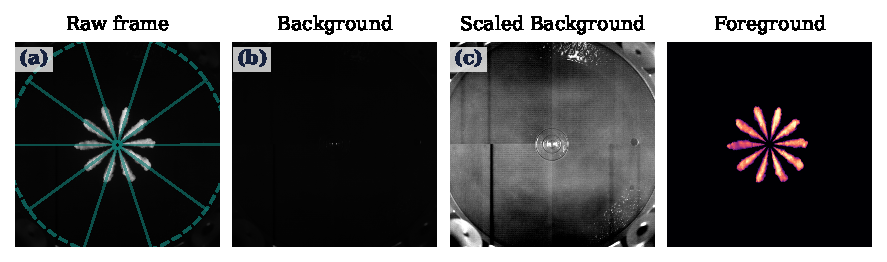
\includegraphics[width=0.98\linewidth]{../images/fig_mie_preproc_background.png}
\caption{Intermediate preprocessing visualization copied from the repository workflow. From left to right: raw frame, estimated background from pre-injection statistics, and log-subtracted foreground.}
\label{fig:mie-preproc-background}
\end{figure}

\subsubsection{Ultra-efficient Sobel high-pass on the CUDA backend}

The second contribution is the explicit edge-enhancing high-pass stage applied directly to the full video cube. In \texttt{arr\_3d\_sobel\_magnitude\_cupy}, Sobel kernels \(K_x\) and \(K_y\) are generated once and applied with \texttt{convolution\_2D\_cupy}:
\[
S_t(x,y)=\sqrt{\left(K_x * F_t\right)^2+\left(K_y * F_t\right)^2}.
\]

A subtler efficiency comes from the rank-1 structure of the Sobel kernel itself. In \texttt{build\_2d\_kernel}, each directional kernel is assembled as an explicit outer product,
\[
K_x = \mathbf{g} \otimes \mathbf{d}_g, \qquad K_y = \mathbf{d}_g \otimes \mathbf{g},
\]
where \(\mathbf{g}\) is a discrete Gaussian envelope and \(\mathbf{d}_g\) is its derivative. An outer-product matrix has algebraic rank exactly one. The function \texttt{\_separable\_factors\_cupy} tests for this automatically: it computes a truncated SVD of the kernel matrix, \(K \approx \sigma_1 \mathbf{u}_1 \mathbf{v}_1^{\top}\), and if the second singular value is negligible the 2-D convolution is replaced by two sequential 1-D passes along the spatial axes. For a \(k \times k\) kernel this reduces the per-pixel multiply-add cost from \(O(k^2)\) to \(O(2k)\). Because the Sobel kernel is rank-1 by construction, the separable path is taken unconditionally at runtime, and both \(K_x\) and \(K_y\) are applied as a pair of 1-D convolutions across the full video cube.

The output is then robust-scaled again and masked by the ring geometry. In implementation terms this matters because it converts a low-contrast grayscale plume into an edge-dominant representation while keeping the whole operation on the CuPy backend. The contribution is not the Sobel operator itself, which is classical, but its integration into a bulk video workflow that avoids repeated host-device copies and prepares every plume for the same downstream geometric treatment \cite{GonzalezWoodsDIP,Szeliski2010Vision}.

\begin{figure}[t]
\centering
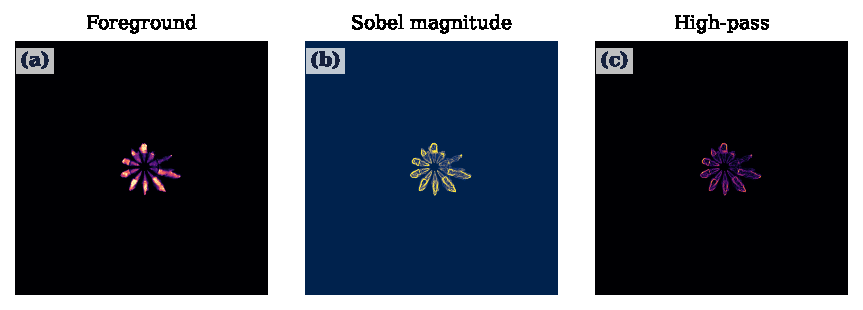
\includegraphics[width=0.98\linewidth]{../images/fig_mie_preproc_sobel.png}
\caption{Repository-generated preprocessing output showing the foreground image, Sobel magnitude, and the final robust-scaled high-pass representation used by the multihole segmentation stage.}
\label{fig:mie-preproc-sobel}
\end{figure}

\subsubsection{Angular density as polar resampling}

After preprocessing, the pipeline does not search for plume directions by contour tracing in Cartesian coordinates. Instead, \texttt{angle\_signal\_density\_auto} performs a polar re-parameterization around the calibrated nozzle center. For every pixel,
\[
\theta(x,y)=\operatorname{atan2}(y-c_y,\;x-c_x)\bmod 360^\circ,
\]
and the per-frame angular signal for bin \(k\) is accumulated as
\[
A_t(k)=\sum_{(x,y)\in \mathcal{B}_k} I_t(x,y), \qquad
D_t(k)=\frac{A_t(k)}{\#\mathcal{B}_k},
\]
where \(\mathcal{B}_k\) is the set of pixels whose angle falls into bin \(k\). In the CuPy implementation, the binning and weighted sums are performed directly on GPU arrays by \texttt{cp.digitize} and \texttt{cp.bincount}. Conceptually, this is a radial collapse of the 2D image into a 1D angular occupancy signal, which is a much more stable object for multihole alignment than raw edge fragments in the original frame \cite{Szeliski2010Vision}.

\subsubsection{FFT-based self-adaptive rotation alignment}

The plume guide angles are then estimated from the periodicity of the angular signal rather than from a fixed offset. Let
\[
\bar{A}(k)=\sum_t A_t(k)
\]
be the time-summed angular profile, and let \(P\) be the known number of plumes. The function \texttt{estimate\_offset\_from\_fft} computes the real FFT of \(\bar{A}\), reads the phase of the plume harmonic \(P\), and converts it to an angular offset
\[
\hat{\phi}_0
=
-\frac{\arg\!\left(\mathcal{F}\{\bar{A}\}[P]\right)}{P}\frac{180^\circ}{\pi}.
\]
This is what makes the alignment self-adaptive: the code uses the observed harmonic phase of the current dataset instead of assuming a manually typed reference angle for every recording. \codepath{mie_multi_hole.py} then constructs plume directions
\[
\phi_p=\frac{360^\circ p}{P}-\hat{\phi}_0, \qquad p=0,\dots,P-1,
\]
and combines them with a triangle-threshold occupancy mask and short-gap filling to reject empty angular sectors. The FFT itself is standard; the contribution here is using the known injector multiplicity to turn the angular-density signal into an automatic plume registration rule \cite{CooleyTukey1965FFT,Szeliski2010Vision}.

The same occupied-angle mask also suggests a simple cone-angle proxy. Treat the bin-wise mask as periodic on \([0,360^\circ)\), merge any \texttt{True} runs that cross the \(0^\circ/360^\circ\) boundary, and convert each contiguous run length from bins to degrees. The resulting angular widths quantify the support occupied by each plume over the full recording. In the notebook figure workflow we report both the total occupied angle and the mean run width; the latter is used as a coarse cone-angle proxy because it summarizes the average angular spread of a plume without requiring a separate edge fit in every frame.

\begin{figure}[t]
\centering
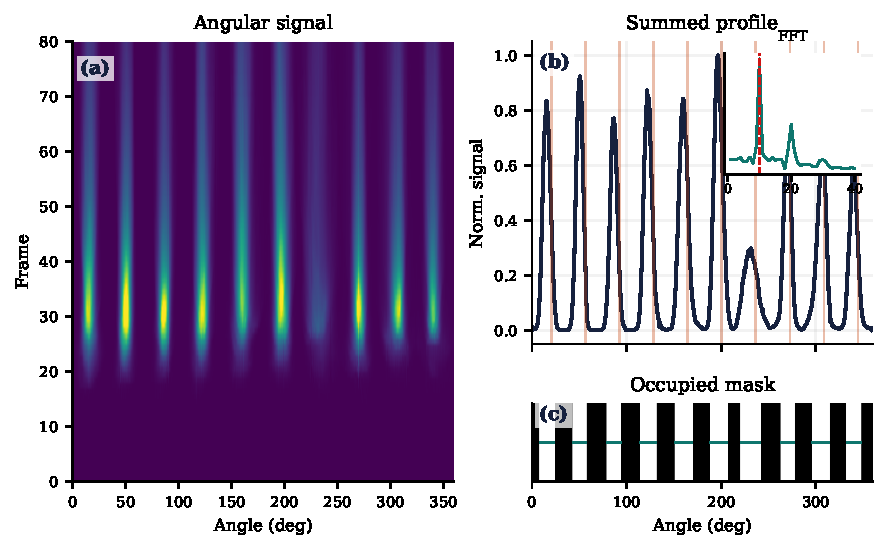
\includegraphics[width=0.98\linewidth]{../images/fig_angular_occupancy.png}
\caption{Processed angular-density outputs from the repository workflow: per-frame angular profiles, time-summed profile with plume guide angles, FFT harmonic content, and the occupied-angle mask used to stabilize multihole alignment.}
\label{fig:angular-occupancy}
\end{figure}

\begin{figure}[t]
\centering
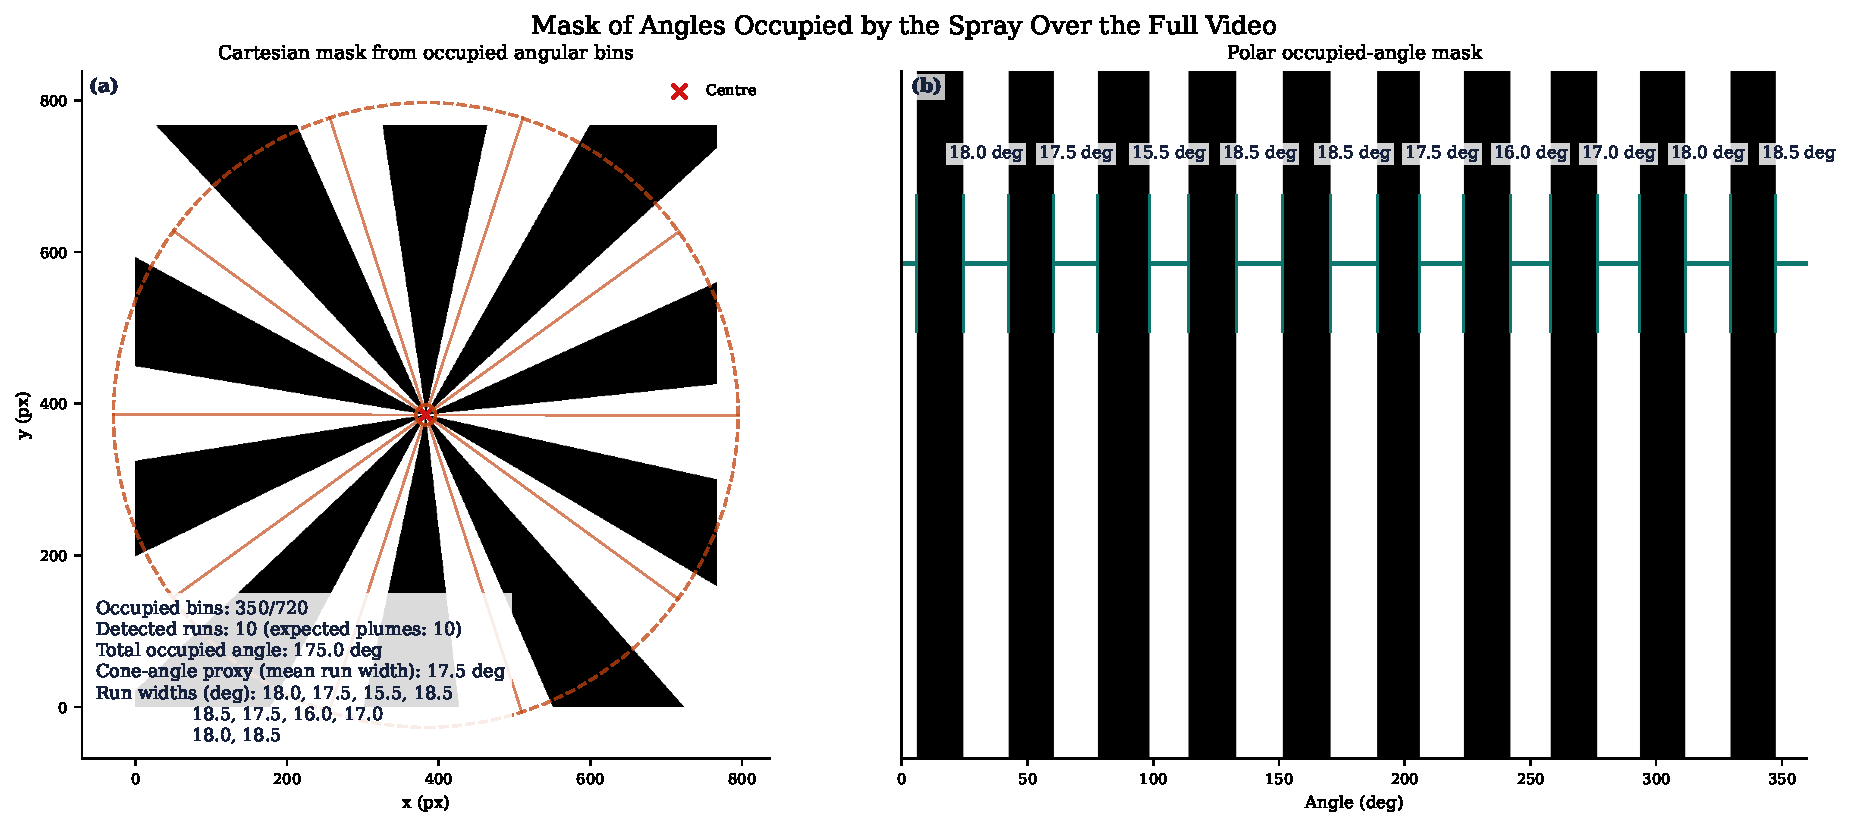
\includegraphics[width=0.98\linewidth]{../images/fig_angular_mask_comparison.png}
\caption{Two coordinate-system views of the same spray-occupied angular support accumulated over the full video. Left: the legacy Cartesian mask obtained by projecting the occupied angular bins back into image space around the nozzle center, together with the total occupied angle and the mean run-width cone-angle proxy. Right: the polar occupied-angle mask used directly in the current workflow, annotated with the angular width of each contiguous occupied segment.}
\label{fig:angular-mask-comparison}
\end{figure}

\subsubsection{Inverse affine mapping and plume-strip extraction}

Once the target angles are known, each plume is remapped into a common nozzle-left strip coordinate system. The forward affine transform built in \texttt{build\_rotation\_affine} is
\[
\begin{bmatrix}
u\\v
\end{bmatrix}
=
\mathbf{A}
\begin{bmatrix}
x\\y
\end{bmatrix}
+\mathbf{b},
\qquad
\mathbf{A}
=
\begin{bmatrix}
\cos\phi_p & \sin\phi_p\\
-\sin\phi_p & \cos\phi_p
\end{bmatrix},
\qquad
\mathbf{b}=\mathbf{t}-\mathbf{A}\mathbf{c},
\]
where \(\mathbf{c}=(c_x,c_y)^\top\) is the nozzle center and \(\mathbf{t}\) places the nozzle at the left edge and mid-height of the output strip. The actual remap uses the inverse relation
\[
\begin{bmatrix}
x_{\mathrm{src}}\\y_{\mathrm{src}}
\end{bmatrix}
=
\mathbf{A}^{-1}
\left(
\begin{bmatrix}
u\\v
\end{bmatrix}
-\mathbf{b}
\right),
\]
implemented in \texttt{build\_affine\_inverse\_maps\_cupy}. For each plume, the map arrays \texttt{mapx} and \texttt{mapy} are precomputed once, and \texttt{remap\_video\_cupy} samples the full video with nearest, bilinear, bicubic, or Lanczos kernels. Importantly, these maps are not spray-intensity images: the pixel value in \texttt{mapx} encodes the source-image \(x\) coordinate sampled for that output pixel, and the pixel value in \texttt{mapy} encodes the corresponding source-image \(y\) coordinate. The multihole pipeline uses a fixed strip size \texttt{OUT\_SHAPE = (outer\_radius/2, outer\_radius)} and applies a triangular plume mask after remapping. This inverse-map formulation is computationally efficient and numerically clean, because every downstream plume metric is measured in the same local coordinate system \cite{Szeliski2010Vision}.

\begin{figure}[t]
\centering
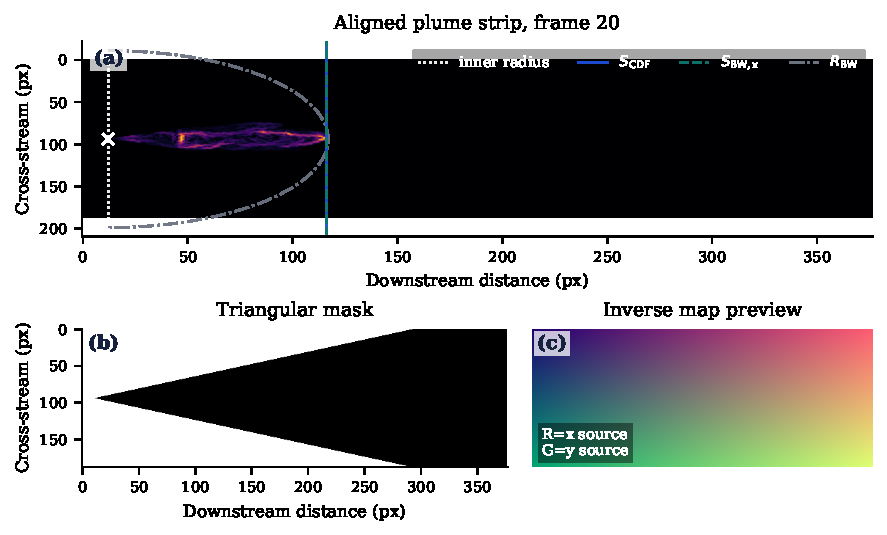
\includegraphics[width=0.98\linewidth]{../images/fig_efficient_rotation.png}
\caption{Repository-generated visualization of the inverse affine remapping stage. Top-left and top-right: \texttt{mapx} and \texttt{mapy}, whose pixel intensities encode the source-image \(x\) and \(y\) coordinates sampled for each output-strip pixel rather than spray brightness. Bottom-left: one rotated plume strip with the orifice-local origin marker at \((H/2,\mathrm{inner\_radius})\), axial penetration overlays plotted at \(\mathrm{inner\_radius}+\)metric, and the polar binary-penetration metric drawn as a radius-\(r\) arc centered at the orifice. Bottom-right: the triangular plume mask used after remapping.}
\label{fig:efficient-rotation}
\end{figure}

\subsubsection{Robust CDF penetration from aligned plume strips}

The penetration estimator is deliberately based on cumulative intensity support instead of on the single brightest pixel or the outermost isolated blob. For each plume strip \(I_p(t,y,x)\), \texttt{penetration\_cdf\_all\_plumes} first collapses the cross-stream direction,
\[
H_p(t,x)=\sum_y I_p(t,y,x),
\]
subtracts a left-edge baseline from each frame, clips negative values, and generates a support mask by automatic thresholding, largest-component cleanup, and binary opening. Within that support, \texttt{penetration\_cdf\_front} forms the axial cumulative distribution
\[
C_p(t,x)=\frac{\sum_{\xi \le x} \tilde{H}_p(t,\xi)}{\sum_{\xi} \tilde{H}_p(t,\xi)+\varepsilon},
\]
and defines the penetration front as the first location satisfying
\[
\hat{x}_p(t)=\min \{x : C_p(t,x)\ge q\},
\]
with \(q\) close to one. The code then enforces monotonicity by \texttt{np.maximum.accumulate}, subtracts the inner radius to express distance from the nozzle annulus, and in \codepath{mie_multi_hole.py} discards traces that show non-physical backward jumps or only very short valid runs. This CDF front is one of the main practical contributions of the workflow: it is much less sensitive to broken leading-edge pixels than a naive max-index definition, while still producing a penetration quantity aligned with standard diesel-spray usage \cite{Dent1971Penetration,HiroyasuArai1990,NaberSiebers1996}.

\subsubsection{Boundary metrics and geometric proxies}

Binarized plume strips are also passed to \texttt{extract\_single\_plume\_features}, which computes several secondary observables. The projected area is
\[
A_p(t)=\sum_{x,y} B_p(t,y,x).
\]
Axial binarized penetration is obtained from the rightmost column whose occupancy exceeds a pixel threshold, while polar penetration is defined from the upper and lower boundary point clouds as
\[
R_p(t)=\max\!\left(
\max_i \sqrt{x_{u,i}^2+y_{u,i}^2},
\max_j \sqrt{x_{l,j}^2+y_{l,j}^2}
\right).
\]
The code also stores a volume-like geometric proxy,
\[
V_p(t)=x_{\mathrm{scale}} \frac{\pi}{4}\sum_x \left(w_u(t,x)+w_l(t,x)\right)^2,
\]
where \(w_u\) and \(w_l\) are the upper and lower half-widths and \(x_{\mathrm{scale}}=1/\cos((180^\circ-\theta_{\mathrm{umb}})/2)\) compensates for umbrella-angle tilt when needed. Cone-angle proxies are computed in two ways: by averaging local boundary angles
\[
\alpha_{\mathrm{avg}}(t)=\overline{\arctan(y_u/x_u)}-\overline{\arctan(y_l/x_l)},
\]
and by fitting fixed-intercept boundary lines and taking
\[
\alpha_{\mathrm{lg}}(t)=\arctan(m_u)-\arctan(m_l).
\]
Near-nozzle opening and closing times are finally inferred from a small detection window close to the injector. These metrics matter because they turn each aligned strip into a compact geometric state vector; however, the downstream modeling in this thesis remains focused on penetration, which is the best-supported target in the archived notebooks \cite{Linne2013SprayImaging,LefebvreMcDonell2017}.

\begin{figure}[t]
\centering
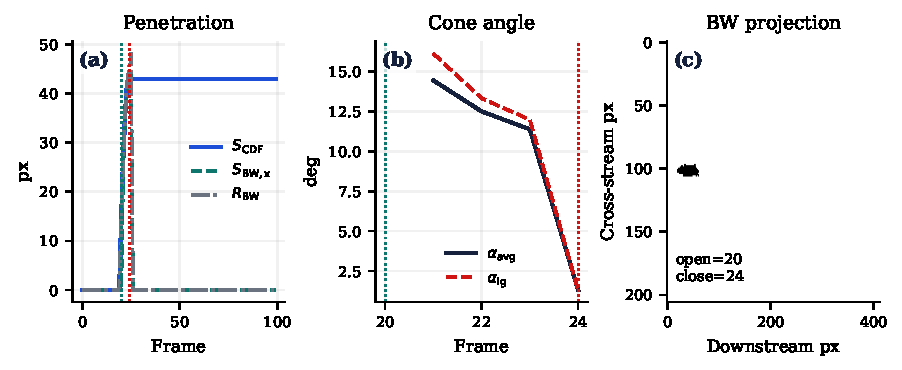
\includegraphics[width=0.98\linewidth]{../images/fig_mie_metrics_summary.png}
\caption{Examples of quantitative outputs produced after plume alignment and binarization: penetration descriptors, plume size, cone-angle proxies, and a representative maximum projection of the binarized plume strip.}
\label{fig:mie-metrics-summary}
\end{figure}

\subsection{Trajectory cleaning and reduced-order fitting in \codepath{MLP/fit_raw_data.py}}

The learned models do not train directly on the raw exported traces. Instead, \texttt{fit\_raw\_data.py} first cleans and time-aligns them. For each plume, the script finds the earliest valid penetration segment, takes the first few positive samples after onset (currently two, controlled by \texttt{NUM\_POINTS\_SOI\_LINEAR\_REGRESSION}), fits a straight line to those early nonzero points, and uses the \(x\)-axis intercept of that line as a subframe opening-delay estimate whenever the fitted slope is positive. If an area-based onset marker is available, that frame anchors the delay scan; otherwise the code falls back to the first positive penetration frame. The resulting raw delay is then clipped to a small median-centered window across plumes so that one anomalous plume does not over-shift the whole group.

That delay estimate is used in two coupled ways. The penetration array itself is shifted left by the nearest integer number of frames, while the aligned time vector retains the fractional residual through the exact offset subtraction. In this way the implementation does not merely discard leading zeros; it performs a plume-onset registration that preserves subframe timing information before the later reduced-order fit. After alignment, the script removes sudden unrealistic jumps, converts pixels to corrected physical length, and flags low-quality fits through a set of rule-based masks.

Each accepted trajectory is then fitted with a smooth two-regime model,
\[
S(t)=\left(1-w(t)\right)k_{\mathrm{sqrt}}\sqrt{t}
+w(t)k_{\mathrm{quarter}}t^{1/4},
\qquad
w(t)=\sigma\!\left(\frac{t-t_0}{s}\right),
\]
where \(k_{\mathrm{sqrt}}\), \(k_{\mathrm{quarter}}\), \(t_0\), and \(s\) are optimized in log space. Concretely, the fitting problem is posed as a robust nonlinear least-squares estimation,
\[
\min_{\theta}
\sum_i \rho_\delta\!\left(S(t_i;\theta)-y_i\right),
\qquad
\theta=
\left[\log k_{\mathrm{sqrt}},\log k_{\mathrm{quarter}},\log t_0,\log s\right],
\]
with the Huber penalty
\[
\rho_\delta(r)=
\begin{cases}
\tfrac{1}{2}r^2, & |r|\le \delta,\\
\delta\left(|r|-\tfrac{1}{2}\delta\right), & |r|>\delta.
\end{cases}
\]
In the implementation, this objective is solved by \texttt{scipy.optimize.least\_squares(..., method="trf", loss="huber")} with \(\delta=1\), while the log-parameterization keeps the fitted gains and transition scale positive \cite{Huber1964,NocedalWright2006}. This fit is not introduced as a baseless convenience curve. It is a reduced-order, data-driven adaptation of the regime-change viewpoint used in diesel spray-penetration literature: Hiroyasu and Arai describe spray development in terms of changing penetration behavior across stages \cite{HiroyasuArai1990}, and later work on start-of-injection transients shows that short injections are difficult to represent well with one rigid empirical expression over the entire trace \cite{ZhouLiYi2021}. That consideration is especially relevant here because the present experiments use pilot diesel injection, for which the near-SOI portion is short, highly transient, and relatively noisy.

The model should therefore be read as a temporal parameterization rather than as an explicit physics law. Its purpose is twofold: to provide believable extrapolation farther from EOI, where the downstream surrogate needs stable targets, and to provide acceptable interpolation near SOI, where the relative error is larger and the apparent early-time physics are harder to constrain from the image trace alone. The sigmoid gate is important for that role. Instead of imposing a hard breakpoint between two empirical branches, it creates a differentiable transition, which keeps the fitted curve smooth and makes it more compatible with the later neural-network stage. In other words, the early transient physics are not forced into a rigid closed-form law here; they are only approximated well enough that the subsequent network can learn the remaining condition-dependent behavior from the full operating-point inputs.

This interpretation becomes clearer when the fit is compared with the extended EOI expressions in the spray literature. The Zhou et al.\ post-EOI model distinguishes the global injection clock \(t\) from the delayed clock \((t-t_i)\), because the late penetration branch is activated only after the end-of-injection dynamics have propagated downstream \cite{ZhouLiLaiWei2019}. The present pipeline handles that delay in two layers. First, the preprocessing stage estimates a plume-wise onset delay from the early linear extrapolation described above and shifts the observed series toward a common \(t\approx 0\) reference. Second, the reduced-order fit itself still does not contain an explicit delayed clock inside the parametric branch. Instead, it uses
\[
w(t)=\sigma\!\left(\frac{t-t_0}{s}\right)
\]
to suppress the quarter-root branch before a learned transition time \(t_0\), and then allows the \(t^{1/4}\) term to dominate only after that transition. This is not algebraically identical to replacing \((t-t_i)^{1/4}\) with \(t^{1/4}\). Rather, it is an engineering reparameterization: on a finite observation window, a delayed fourth-root branch can often be represented adequately by a gated unshifted fourth-root branch with adjusted amplitude and transition location, especially when the early part of that branch is strongly attenuated by \(1-w(t)\) or \(w(t)\) near zero. In that sense, the delayed physical clock is absorbed into the learned switching parameters \((t_0,s)\) and into the branch amplitudes rather than being imposed as a fixed known constant.

I therefore consider the engineering approach reasonable for the stated objective of this thesis, with one clear boundary. It is reasonable because the fit is used as a smooth compressor of noisy trajectories, not as a final mechanistic spray law; it keeps the curve differentiable for later learning; and it leaves the operating-condition dependence to the neural network instead of forcing every physical effect into the closed-form fit. The boundary is that this justification should be presented as a reduced-order surrogate motivated by empirical penetration theory, not as proof that the shifted-time physics have disappeared. A stricter physics-oriented study would compare the present fit directly against a branch written explicitly in \((t-t_i)\) and report the ablation.

The archived local analysis supports this interpretation. The exploratory notebooks in \texttt{MLP/interpretatable\_test} explicitly describe the model as a Hiroyasu--Arai-inspired two-branch blend, while \texttt{fitted\_stats\_analysis.ipynb} and the archived clean-fit CSV tables show that \(k_{\mathrm{sqrt}}\) behaves more like an optional shape descriptor than a uniformly stable physical coefficient. Across the current clean-fit archive, the square-root branch amplitude at the fitted transition time is smaller than half of the quarter-root branch for the large majority of accepted rows, so many successful fits effectively degenerate toward a quarter-root-dominated curve. This is acceptable for the intended use: the physical drivers are later given directly to the neural network, while the fit itself remains self-adaptive and physics-light. In the archived production outputs under \texttt{MLP/synthetic\_data}, 105\,594 of 123\,902 candidate rows are marked as successful by the raw nonlinear fit, corresponding to a practical success rate of about \(85\%\) before the stricter post-fit masking stage. The practical purpose of this fit is therefore not to claim a universal penetration law, but to compress noisy plume trajectories into smooth, differentiable, and trainable targets while still preserving the dataset's heteroscedastic variation for the later learning stages.

The stricter post-fit masking stage is also an important part of the engineering contribution. In \texttt{apply\_filter\_masking}, the script first forms a far-time penetration proxy by evaluating the fitted curve at \(t_{\mathrm{far}}=\SI{5}{ms}\). The row is retained only if that far-time value remains inside a broad physically plausible window and if the fit parameters pass basic sanity checks on \(t_0\), \(s\), point count, and fit cost. The code then computes robust grouped outlier scores using the median absolute deviation,
\[
z_{\mathrm{robust}}(x)=0.6745\,\frac{x-\operatorname{median}(x)}{\operatorname{MAD}(x)+\epsilon},
\qquad
\operatorname{MAD}(x)=\operatorname{median}\!\left(\lvert x-\operatorname{median}(x)\rvert\right),
\]
applied to \(t_0\), \(\log(1+\mathrm{RMSE})\), and \(\log(1+\mathrm{cost\_per\_point})\) within each file group. Rows with \(|z_{\mathrm{robust}}|>3\) on any of those diagnostics are marked as outliers and excluded from the clean archive. This matters for the later neural-network stages because it removes evidently unstable fits before they can distort the training distribution. The result is a deliberately conservative curation step: the network does not see every fitted row, only those trajectories that remain numerically plausible both near the fitted transition and at a fixed far time.

\subsection{Sparse-feature instability in the direct-feature baseline}

Before the v2 architecture was finalised, an earlier nine-feature MLP was trained with direct pressure and diameter inputs. A systematic diagnostic documented in \codepath{MLP/v1\_direct\_feature\_training/slides\_sparse\_feature\_instability} revealed a structural pathology. Nozzle diameter has only six levels in the dataset and is not uniformly available across pressure combinations: all six diameter levels appear only on the family $(P_{\mathrm{inj}}=\SI{2000}{bar},\;P_{\mathrm{cb}}=4,\;P_{\mathrm{ch}}\in\{5,10,15\}\,\si{bar})$. Injection pressure has four levels. Because a smooth MLP treats these as continuous inputs, it can produce derivative structure along the diameter and pressure axes that the data simply do not constrain. Dense MLP sweeps over diameter showed five to six gradient sign changes with worst-secant-deviation ratios below one and curvature norms of order~$10^7$; injection pressure showed unsupported extrapolation on thinly supported slices. This pathology is a structural consequence of the sparse-feature geometry and persists across time. Adding regularisation would suppress instability at the cost of useful capacity everywhere; the underlying problem is that a smooth MLP is being asked to learn a physically meaningful continuous law from an effectively discrete sample grid. The v2 architecture therefore addresses this at the source.

\subsection{Engineered-feature design in \codepath{MLP/v2\_engineered\_feature}}

The v2 surrogate replaces the four weakly supported pressure and diameter inputs with a single hard scaling group derived from the Hiroyasu--Arai post-breakup branch \cite{HiroyasuArai1990}. From the post-breakup form
\[
S(t)\;\propto\;K_p\!\left(\frac{\Delta P}{\rho_a}\right)^{1/4}d_n^{1/2}\,t^{1/2},
\]
all dependence on injection pressure, chamber pressure, chamber density, and nozzle diameter collapses to one per-condition length scale
\[
A\;=\;\left(\frac{\Delta P}{\rho_a}\right)^{1/4}d_n^{1/2},
\]
computed in \texttt{engineered\_feature\_common.build\_canonical\_feature\_table} from the test-matrix JSON. For Nozzle1--Nozzle8 the chamber density is taken directly from \texttt{chamber\_density\_kg\_per\_m3}; for DS300, where only \texttt{chamber\_pressure\_bar} is recorded, $\rho_a$ is reconstructed from the linear law $\rho_a=\SI{5}{kg/m^3}\times P_{\mathrm{ch}}/\SI{4.42}{bar}$ calibrated against the Nozzle1--8 entries.

The four sparse columns are removed entirely, leaving two feature-vector variants. The five-feature \texttt{a\_only} variant
\[
[\,t_{\mathrm{norm}},\;\theta_{\mathrm{tilt},z},\;n_{\mathrm{plumes},z},\;t_{i,z},\;P_{\mathrm{cb},z}\,]
\]
treats $A$ as a target divisor only. The six-feature \texttt{a\_plus\_log\_a} variant additionally contains $\log A_z$ as a one-dimensional residual axis. The training target is reparameterised to the non-dimensional penetration $\hat{S}(t)=S(t)/A$; the network predicts $\hat{\mu}$ and $\log\hat{\sigma}^2$, and physical predictions are recovered at inference as $\mu_S=A\,\hat{\mu}$ and $\sigma_S=A\,\hat{\sigma}$.

Before any optimisation, \texttt{run\_pretrain\_collapse\_check} tests the scaling assumption on the actual dataset: it divides each trajectory by its own $A$, reports the per-time-slice variance reduction, and computes a linear-regression $R^2$ of $\hat{S}(t)$ on the kept features. In the archived runs the check passed with a median post-\SI{0.5}{ms} variance reduction of~59.5\% (collapse ratio~0.405) and a sparse-feature $R^2$ dropping from~0.34 on $S$ to~0.14 on $\hat{S}$, confirming that $A$ accounts for the dominant diameter and pressure variation and that the network is learning only the residual structure on the dense, well-supported axes. If the check fails, training aborts by default, making the physical prior falsifiable rather than asserted.

The driver scripts \texttt{train\_stage1\_mse.py} and \texttt{train\_stage2\_nll.py} also introduce group-aware data splits: \texttt{assign\_splits\_by\_group} assigns whole \texttt{sample\_group\_id} groups to train, validation, and test, preventing leakage between curves that share an operating point. Stage~2 warm-starts strictly from a Stage-1 engineered run directory and reuses its scaler state, guaranteeing consistent variant choice and $A$-scaling across both stages.

\subsection{Stage-1 MSE baseline on the non-dimensional target}

Stage~1 trains a deterministic mean model on a representative-trajectory subset. For each file-level operating-condition group, the fitted curve is evaluated at $t_{\mathrm{far}}=\SI{5}{ms}$, the group-median penetration is computed, and the nearest row is kept as the stage-1 representative. In the archived run \codepath{stage1\_engineered\_mse\_a\_only\_20260410\_020317} this produced 526~representative trajectories, split by group into training, validation, and test sets.

The loss applied to the non-dimensional target $\hat{S}$ is
\[
\begin{aligned}
\mathcal{L}_{\mathrm{stage1}}
=\;&\operatorname{MSE}\!\left(\hat{\mu},\hat{S}\right)
+\lambda_{\mathrm{var}}
\mathbb{E}\!\left[\left(\log \hat{\sigma}^2-c_0\right)^2\right]\\
&+\lambda_{1}
\mathbb{E}\!\left[\operatorname{ReLU}\!\left(-\frac{\partial \mu_S}{\partial t}\right)^2\right]
+\lambda_{2}
\mathbb{E}\!\left[g(t)\operatorname{ReLU}\!\left(\frac{\partial^2 \mu_S}{\partial t^2}\right)^2\right],
\end{aligned}
\]
where $c_0=-2$ is the log-variance prior centre, $g(t)=\sigma((t-t_c)/\tau_c)$ gates the concavity penalty to activate after the transient region, and the derivative penalties are evaluated on the physical reconstruction $\mu_S=A\,\hat{\mu}$ so that the monotonicity and concavity constraints apply at the observable scale. The network is a three-hidden-layer MLP with dimensions $[512,512,128]$, GELU activations, dropout~0.3, and AdamW optimisation with gradient clipping and early stopping on validation loss. The run achieved a best validation MSE (on the scaled target) of~18.94 at epoch~115 and a test physical MAE of~\SI{8.1}{mm}. The run directory contains \codepath{best\_model\_stage1.pt}, \codepath{scaler\_state.json}, epoch and iteration loss logs, and a \codepath{pretrain\_collapse\_summary.png}.

\subsection{Stage-2 NLL heteroscedastic extension}

Stage~2 warm-starts from the Stage-1 checkpoint and expands the training set to all filtered trajectories, replacing the MSE data-fit term with a heteroscedastic Gaussian NLL on the scaled target:
\[
\mathcal{L}_{\mathrm{stage2}}
=
\underbrace{\mathbb{E}\!\left[
\frac{1}{2}\left(
\log \hat{\sigma}^2
+\frac{(\hat{S}-\hat{\mu})^2}{\hat{\sigma}^2}
\right)\right]}_{\text{heteroscedastic NLL on }\hat{S}}
+\lambda_{1}
\mathbb{E}\!\left[\operatorname{ReLU}\!\left(-\frac{\partial \mu_S}{\partial t}\right)^2\right]
+\lambda_{2}
\mathbb{E}\!\left[g(t)\operatorname{ReLU}\!\left(\frac{\partial^2 \mu_S}{\partial t^2}\right)^2\right],
\quad\hat{\sigma}^2=\exp(\log\hat{\sigma}^2)+\varepsilon.
\]
The derivative penalties remain on the physical-space reconstruction $\mu_S=A\,\hat{\mu}$. The row table expands to 14,594~filtered trajectories, retaining all rows that pass the fit-level masks and a far-time z-score filter on group-wise spread. The split is assigned at the \texttt{sample\_group\_id} level rather than at the individual plume-trajectory level, so trajectories from the same physical case do not leak across train, validation, and test partitions. With 512 time samples per trajectory over \SIrange{0}{5}{ms}, the archived Stage-2 table contains 7,472,128 pointwise samples: 10,333 trajectories from 370 groups for training, 2,092 trajectories from 78 groups for validation, and 2,169 trajectories from 78 groups for testing.

The retained trajectories span the dominant operating range in the archive: control back-pressure from 1 to \SI{4}{bar}, injection pressure from 1,400 to \SI{2,200}{bar}, injection duration from 380 to \SI{1,200}{\micro\second}, and fitted far-time penetration from \SI{58.1}{mm} to \SI{202.6}{mm}. The Stage-2 model therefore does not only learn a single median curve; it sees the remaining within-condition plume and repeat variation after outlier removal. The heteroscedastic output is used to separate two effects that would be conflated by a pure MSE objective: the conditional mean trajectory and the conditional spread around that mean.

Training reuses the Stage-1 feature mapping and scaler state. The input vector remains \([\texttt{time\_norm\_0\_5ms},\theta_z,N_{\mathrm{plume},z},\Delta t_{\mathrm{inj},z},p_{\mathrm{back},z}]\), the architecture remains the three-hidden-layer MLP with dimensions $[512,512,128]$, and the network is warm-started from \codepath{best\_model\_stage1.pt}. The Stage-2 run uses AdamW with learning rate \(8\times10^{-4}\), weight decay \(10^{-4}\), batch size~96, gradient clipping at norm~1.0, log-variance bounds \([-10,6]\), and early stopping with patience~35. Thus the only intentional change in the data-fit term is the replacement of deterministic MSE by the Gaussian NLL and its learned variance output.

\begin{table}[t]
\centering
\footnotesize
\setlength{\tabcolsep}{3pt}
\begin{tabular}{|L{0.20\linewidth}|L{0.08\linewidth}|L{0.14\linewidth}|L{0.13\linewidth}|L{0.12\linewidth}|L{0.12\linewidth}|}
\hline
Record from \codepath{epoch\_loss.csv} & Epoch & Pointwise samples & Loss / scaled NLL & Physical MAE & Mean predicted std. \\
\hline
Train at best validation epoch & 66 & 5{,}290{,}496 & 2.156 / 2.148 & \SI{9.83}{mm} & \SI{12.27}{mm} \\
Validation, best checkpoint & 66 & 1{,}071{,}104 & 2.038 / 2.038 & \SI{8.81}{mm} & \SI{11.71}{mm} \\
Validation, stopping epoch & 101 & 1{,}071{,}104 & 2.053 / 2.053 & \SI{8.97}{mm} & \SI{12.11}{mm} \\
Test, restored best checkpoint & 101 & 1{,}110{,}528 & 2.083 / 2.083 & \SI{9.18}{mm} & \SI{11.44}{mm} \\
\hline
\end{tabular}
\caption{Epoch-level Stage-2 loss summary from \codepath{MLP/runs\_mlp/stage2\_engineered\_nll\_a\_only\_20260410\_020607/epoch\_loss.csv}. The test row is written after early stopping, but the model weights are restored to the best validation checkpoint before test evaluation.}
\label{tab:stage2-epoch-loss}
\end{table}

Table~\ref{tab:stage2-epoch-loss} shows that the best validation NLL is reached at epoch~66, while early stopping terminates the run at epoch~101 after no better validation loss is found. The held-out test MAE of \SI{9.18}{mm} is close to the validation MAE, and the mean predicted standard deviation of \SI{11.44}{mm} remains larger than the point-error scale. This is the desired behaviour for this stage: the model is not forced to explain all residual plume-to-plume variation through the mean function, but instead assigns a nonzero conditional uncertainty that can be used by the later impingement and distillation stages. The run directory contains \codepath{best\_model\_stage2.pt}, \codepath{scaler\_state.json}, \codepath{row\_table.csv}, \codepath{epoch\_loss.csv}, \codepath{iteration\_loss.csv}, \codepath{test\_summary.csv}, and \codepath{stage2\_loss\_curves.png}; \codepath{best\_model\_stage2.pt} serves as the teacher checkpoint for the subsequent distillation stage.

\subsection{Raw-CDF distillation and onset refinement}

The NLL stage produces well-calibrated heteroscedastic predictions on the fitted training targets, but the fitted curves are not equally faithful over the whole time axis. Near the onset of injection the absolute penetration is small, and any timing offset, fit-delay ambiguity, or smoothness prior produces a relatively large fractional error, so the earliest segment of each predicted curve is dominated by the fitted-target prior rather than by directly observed raw plume dynamics. Figure~\ref{fig:stage2-toy-inference-early-time} illustrates this in a representative toy-inference sweep.

\begin{figure}[t]
\centering
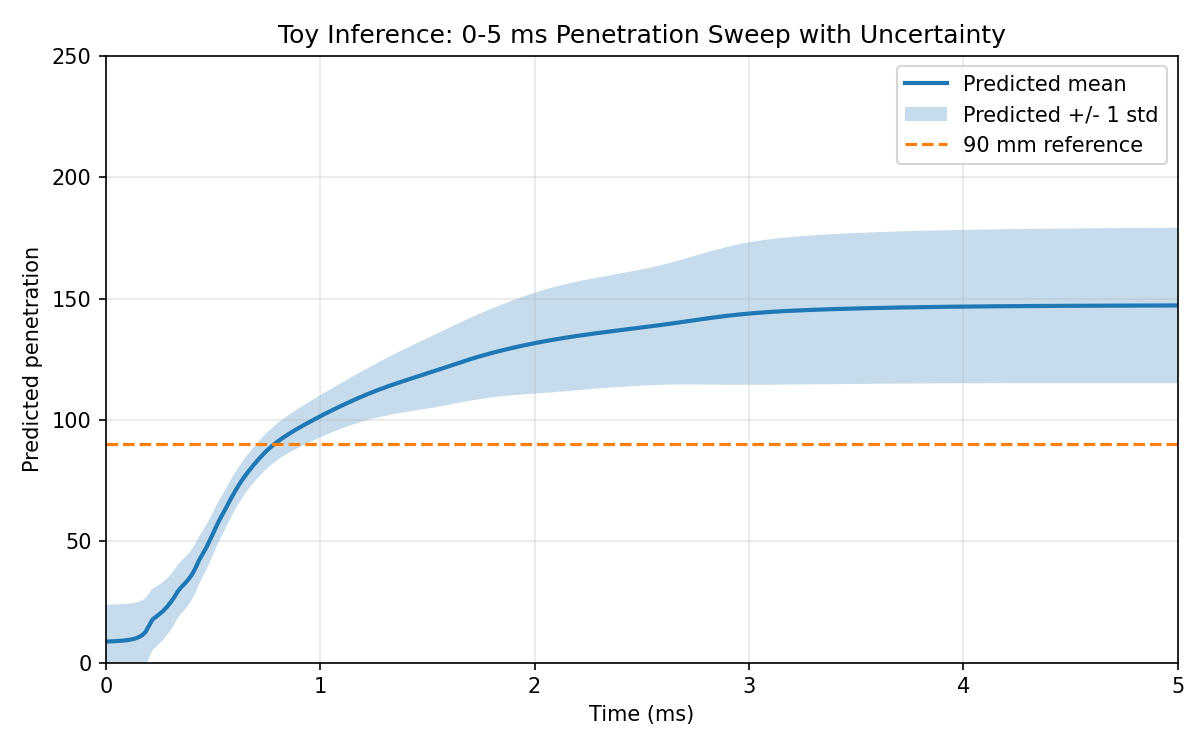
\includegraphics[width=0.82\linewidth]{images/stage2_toy_inference_2000bar_5bar.png}
\caption{Toy inference of the stage-2 NLL model for a representative \(\SI{2000}{bar}\), \(\SI{5}{bar}\) case. The prediction is smooth and well-behaved overall, but the earliest part of the trajectory is still shaped primarily by the fitted-target prior, motivating the subsequent distillation refinement.}
\label{fig:stage2-toy-inference-early-time}
\end{figure}

To refine the early-time dynamics against raw CDF observations while preventing collapse in the late-time sparse regime, a knowledge-distillation stage is implemented in \codepath{MLP/distillation\_plus\_raw\_series.py} and archived under \codepath{runs\_mlp/distill\_cdf\_onset\_v2\_20260410\_103413}. The Stage-2 NLL model serves as a fixed teacher; the student network inherits the teacher weights and is further trained on raw CDF together with teacher guidance.

\textbf{CDF coverage regimes.}  Because the raw CDF series are right-censored (by $t\approx\SI{3}{ms}$ many operating conditions have lost more than 70\% of their measurements), direct raw supervision cannot be applied uniformly in time. For each operating-condition group, raw observations are binned in $\Delta t=\SI{0.1}{ms}$ intervals over $[0,5]\,\si{ms}$, and the smoothed sample count per bin determines three mutually exclusive regimes: \texttt{raw\_reliable} (smoothed coverage $\geq70\%$ of peak), \texttt{raw\_uncertain} (coverage between 20\% and 70\%), and \texttt{teacher\_only} (coverage below 20\% or fewer than 4 samples per bin). Transitions require at least two consecutive bins in a regime to prevent isolated dips from triggering premature regime changes.

\textbf{Supervision weights.}  Each grid point receives two independent weight channels:

\begin{center}
\begin{tabular}{lcc}
\toprule
Regime & Raw weight $w_{\mathrm{raw}}$ & KD weight $w_{\mathrm{kd}}$ \\
\midrule
\texttt{raw\_reliable}  & 1.0 & 0.25 \\
\texttt{raw\_uncertain} & 0.0 & 1.0  \\
\texttt{teacher\_only}  & 0.0 & 0.75 \\
\bottomrule
\end{tabular}
\end{center}

Both channels are further modulated by a global time-bin rebalancing weight (inverse-frequency, clipped to $[0.5,2.0]$). In \texttt{raw\_reliable} bins, raw NLL is the primary signal with mild KD regularisation. In \texttt{raw\_uncertain} bins, raw supervision is dropped and teacher KL dominates. In \texttt{teacher\_only} bins, the KD weight is slightly reduced to acknowledge teacher extrapolation uncertainty.

\textbf{Composite loss.}  The training objective is
\[
\mathcal{L} = \mathcal{L}_{\mathrm{raw}} + \mathcal{L}_{\mathrm{KD}} + \lambda_{\mathrm{onset}}\,\mathcal{L}_{\mathrm{onset}} + \lambda_{\mathrm{anchor}}\,\mathcal{L}_{\mathrm{anchor}} + \lambda_{d_1}\,P_{d_1} + \lambda_{d_2}\,P_{d_2},
\]
where $\mathcal{L}_{\mathrm{raw}}$ is the Gaussian NLL on physical $(\mu,\sigma^2)$ against raw CDF targets weighted by $w_{\mathrm{raw}}$; $\mathcal{L}_{\mathrm{KD}}$ is the forward KL divergence $\mathrm{KL}(q_{\mathrm{student}}\|p_{\mathrm{teacher}})$ in physical space weighted by $w_{\mathrm{kd}}$ and a teacher confidence factor
\[
w_{\mathrm{conf}}(t) = \mathrm{clamp}\!\left(\frac{\sigma_{\mathrm{ref}}}{\sigma_{\mathrm{teacher}}(t)},\;0.25,\;1.0\right),\quad\sigma_{\mathrm{ref}}=\SI{10}{mm};
\]
$\mathcal{L}_{\mathrm{onset}}$ is a BCE loss on a new onset logit output against a ramp target $\min(t/t_{\mathrm{ramp}},1)$ active only for $t\leq\SI{0.2}{ms}$ ($\lambda_{\mathrm{onset}}=0.1$); $\mathcal{L}_{\mathrm{anchor}}$ is a quadratic penalty pulling $\mu(t\approx0)$ toward zero, ramping down over the first \SI{0.15}{ms} ($\lambda_{\mathrm{anchor}}=0.01$); $P_{d_1}=\operatorname{ReLU}(-\Delta\mu)^2$ enforces monotonicity; and $P_{d_2}=\operatorname{ReLU}(+\Delta^2\mu)^2$ enforces concavity for $t\geq\SI{0.5}{ms}$.

\textbf{Student architecture.}  The student is a three-output MLP extending the teacher's two outputs $[\hat\mu,\;\log\hat\sigma^2]$ with an onset logit. All shared layers are copied from the teacher checkpoint; the final linear row for the onset head is initialised to zero (sigmoid $\to0.5$). All losses are computed in physical space by multiplying student and teacher outputs by the per-sample $A$ before evaluating $\mathcal{L}_{\mathrm{KD}}$, $\mathcal{L}_{\mathrm{raw}}$, and the shape priors.

\textbf{Training and results.}  The student is optimised with AdamW at $\mathrm{lr}=3\times10^{-3}$ with gradient clipping at norm~1.0 and early stopping with patience~20. In the archived run \codepath{distill\_cdf\_onset\_v2\_20260410\_103413}, the best validation loss was~2.327 at epoch~55 (val raw NLL~2.256, val KD KL~0.018, val onset BCE~0.308). On the held-out test set: raw NLL~2.29, KD KL~0.019, onset BCE~0.309, with negligible derivative penalties ($P_{d_1}\approx6.5\times10^{-7}$, $P_{d_2}\approx2.3\times10^{-5}$). The run directory contains \codepath{best\_model\_refinement.pt} and \codepath{loss\_curves.png}; Figure~\ref{fig:distillation-loss} shows the training curves.

\begin{figure}[t]
\centering
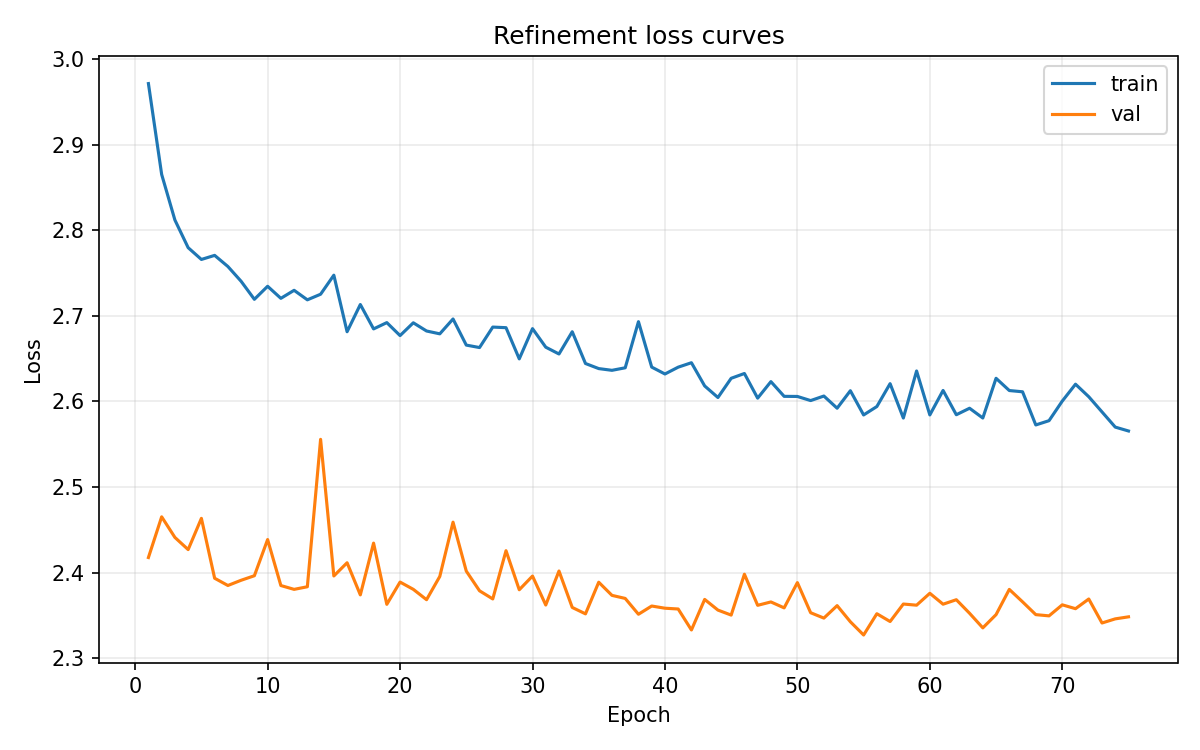
\includegraphics[width=0.92\linewidth]{images/distillation_loss_curves.png}
\caption{Distillation stage training curves from \codepath{runs\_mlp/distill\_cdf\_onset\_v2\_20260410\_103413/loss\_curves.png}. The composite loss converges to a best validation of~2.327 at epoch~55.}
\label{fig:distillation-loss}
\end{figure}

\subsection{Prototype inference notebook}

The notebook \codepath{MLP/toy_inference_from_run.ipynb} demonstrates how a stored run directory can be loaded for manual inference. The archived output shows that, when pointed to the stage-2 run directory above, the prototype resolves the available checkpoint as \codepath{best_model_stage1.pt}. It then generates mean and standard-deviation curves and overlays them on simple geometric masks.

This prototype is useful as a proof of concept because it exercises the scaling state, the trained network interface, and a simple downstream visualization path. It is not used here as evidence for a finished collision-detection product.

\section{Results}

\subsection{Extracted and cleaned trajectory assets}

The current workspace contains ten campaign folders under \texttt{MLP/synthetic\_data} and 295 cleaned fitted CSV files under the corresponding \texttt{clean} subfolders. This means the image-processing side of the workflow is not merely a draft: it has already produced a sizeable archive of cleaned penetration-oriented assets from multiple campaign folders.

Figure~\ref{fig:clean-fit-example} shows a representative cleaned penetration plot from the archived output directory. The solid curves are cleaned trajectories and the dashed curves are the fitted reduced-order curves from the \texttt{cdf} pathway. The figure illustrates the practical role of \texttt{MLP/fit\_raw\_data.py}: smooth the raw plume-wise trajectories enough that they can be modeled later without discarding their main temporal structure.

\begin{figure}[t]
\centering
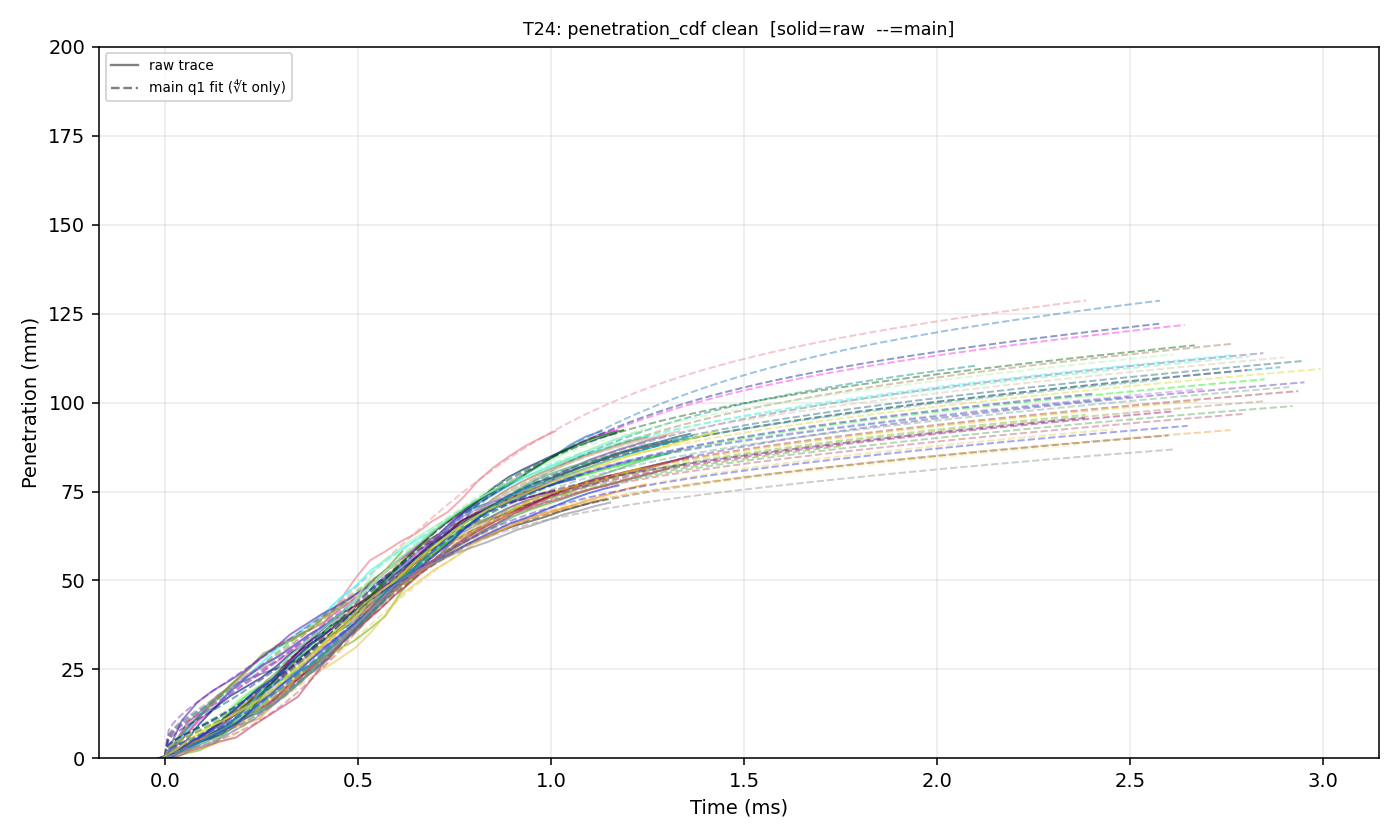
\includegraphics[width=0.92\linewidth]{images/representative_clean_fit.png}
\caption{Representative cleaned trajectories and fitted curves from \codepath{MLP/synthetic_data/BC20241003_HZ_Nozzle1/cdf/plots_clean/T1.png}. The figure is used here as direct evidence that the trajectory-cleaning and fitting stage has already produced reusable penetration targets.}
\label{fig:clean-fit-example}
\end{figure}

\subsection{Stage-1 MSE baseline}

The Stage-1 MSE baseline establishes the representative-trajectory mean model. Table~\ref{tab:model-summary} summarises the quantitative evidence across all three training stages.

\begin{figure}[t]
\centering
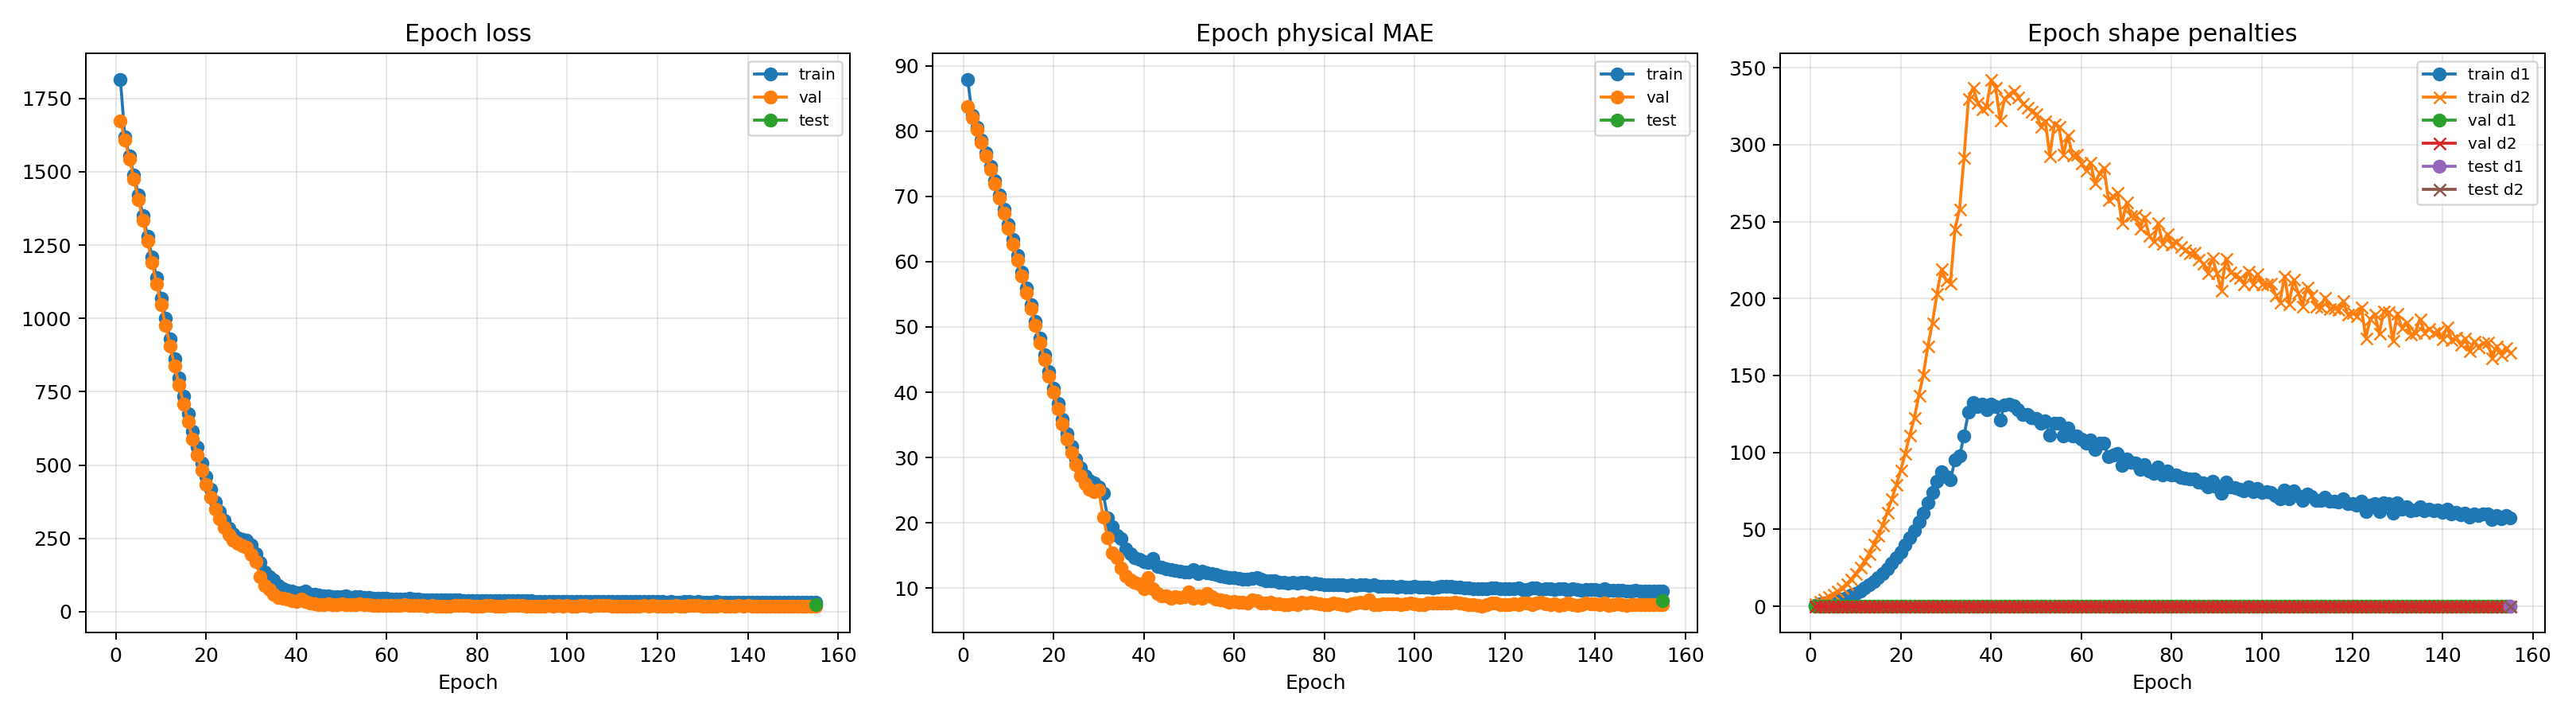
\includegraphics[width=0.92\linewidth]{images/stage1_loss_curves.png}
\caption{Stage-1 training curves from \codepath{MLP/runs\_mlp/stage1\_engineered\_mse\_a\_only\_20260410\_020317/stage1\_loss\_curves.png}.}
\label{fig:stage1-loss}
\end{figure}

The archived run \codepath{stage1\_engineered\_mse\_a\_only\_20260410\_020317} trained on 526~representative trajectories, selected as the group-median curve at $t=\SI{5}{ms}$ after fit-level masking. The run achieved a best validation MSE of~18.94 on the scaled target at epoch~115, with a test physical MAE of~\SI{8.1}{mm}. The pretrain collapse report confirms a 59.5\% post-\SI{0.5}{ms} variance reduction under the $A$-scaling hypothesis, validating that the scaling accounts for the dominant diameter and pressure variation before the network sees any data. The run directory contains \codepath{best\_model\_stage1.pt}, \codepath{scaler\_state.json}, epoch and iteration loss logs, and \codepath{pretrain\_collapse\_summary.png}.

\subsection{Stage-2 NLL extension}

The Stage-2 run expands the training set to all 14,594~filtered trajectories and replaces the MSE objective with heteroscedastic NLL, warm-starting from the Stage-1 checkpoint.

\begin{figure}[t]
\centering
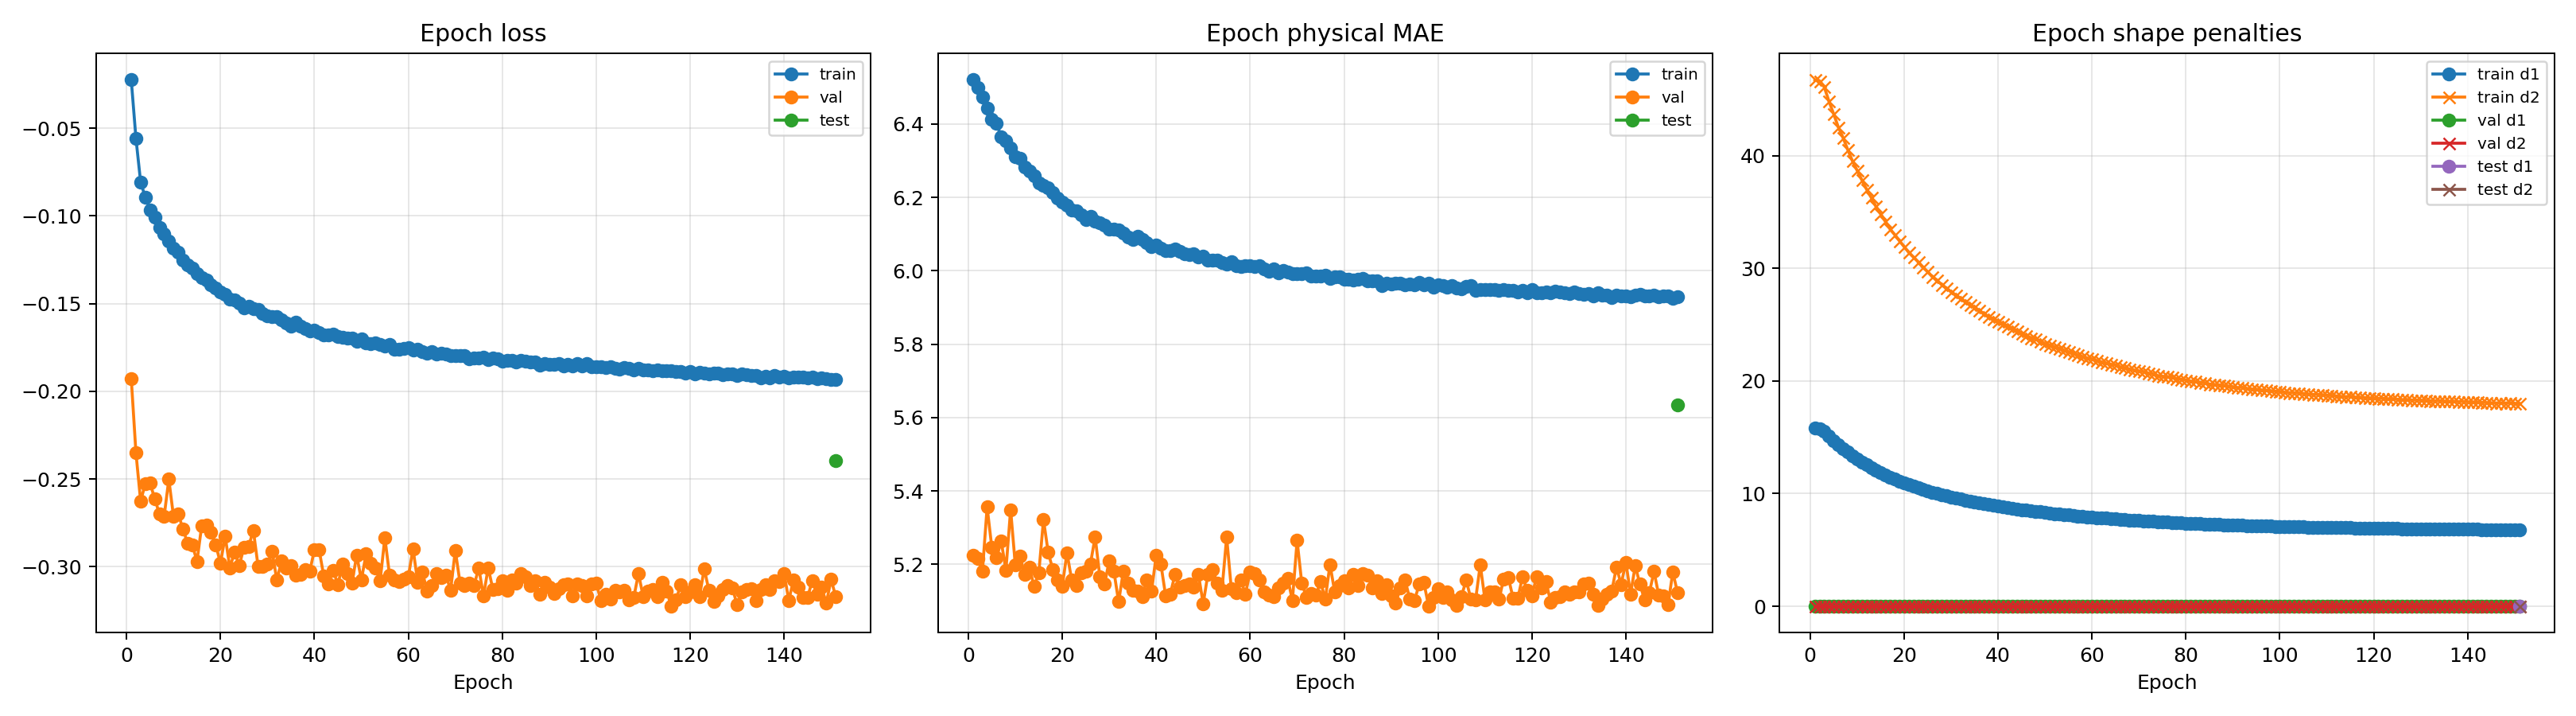
\includegraphics[width=0.92\linewidth]{images/stage2_loss_curves.png}
\caption{Stage-2 training curves from \codepath{MLP/runs\_mlp/stage2\_engineered\_nll\_a\_only\_20260410\_020607/stage2\_loss\_curves.png}.}
\label{fig:stage2-loss}
\end{figure}

The archived run \codepath{stage2\_engineered\_nll\_a\_only\_20260410\_020607} reached a best validation NLL of~2.038 at epoch~66. On the held-out test set the physical MAE is~\SI{9.2}{mm} and the mean predicted standard deviation is~\SI{11.4}{mm}, indicating that the model assigns nontrivial uncertainty broader than the MAE --- consistent with genuine conditional variability in the filtered dataset. The run directory contains \codepath{best\_model\_stage2.pt} and serves as the teacher checkpoint for the distillation stage.

\subsection{Tuned distillation refinement}

The final stage archives a student that has been refined toward raw CDF observations. The latest tuned run \codepath{distill\_cdf\_onset\_v2\_loss\_tuned\_conservative\_20260418\_114747} evaluates to an overall RMSE of~\SI{6.60}{mm} (NRMSE 6.88\%) and a mean absolute error of~\SI{4.81}{mm} across 14,972~trajectories. Loss-tuning significantly reduces the global under-prediction bias from \SI{-1.29}{mm} to \SI{-0.40}{mm} compared to earlier baselines, particularly mitigating early-SOI errors in DS300. The heteroscedastic uncertainty intervals remain reliably conservative (73.56\% coverage at 1$\sigma$, 96.93\% at 2$\sigma$). Ablation studies confirm that lowering KD strength in reliable raw-observation bins fixes the main bias direction, validating the hypothesis that overly strong teacher distillation conflicts with deterministic raw observations. The run directory contains \codepath{best\_model\_refinement.pt} and ablation summaries.

\begin{table}[t]
\centering
\begin{tabular}{|L{0.20\linewidth}|L{0.18\linewidth}|L{0.20\linewidth}|L{0.20\linewidth}|}
\hline
Stage & Data evidence & Best validation result & Current status \\
\hline
Image-processing and fitting & 10 campaign folders and 295 cleaned fitted CSV files under \codepath{MLP/synthetic\_data} & Representative cleaned/fitted trajectory plots available & Completed and auditable \\
\hline
Stage 1 MSE baseline & 526 representative rows, group-aware split & Val MSE~18.94 at epoch~115; test MAE~\SI{8.1}{mm} & Completed with \codepath{best\_model\_stage1.pt} \\
\hline
Stage 2 NLL extension & 14,594 filtered rows, warm-started from Stage~1 & Val NLL~2.038 at epoch~66; test MAE~\SI{9.2}{mm} & Completed with \codepath{best\_model\_stage2.pt} \\
\hline
Tuned distillation & Raw CDF + KD ablation, regime-dependent supervision & RMSE~\SI{6.60}{mm}, Bias~\SI{-0.40}{mm} & Completed with \codepath{best\_model\_refinement.pt} \\
\hline
Prototype inference & Archived notebook outputs from \codepath{MLP/toy\_inference\_from\_run.ipynb} & Mean/std prediction plots and simple overlap calculations & Prototype only, not a validated product \\
\hline
\end{tabular}
\caption{Evidence summary of the completed project stages.}
\label{tab:model-summary}
\end{table}

\subsection{Prototype inference notebook}

The prototype inference notebook demonstrates a plausible deployment direction rather than a final scientific endpoint. Its archived outputs show that it loads run metadata, produces predicted mean and standard-deviation curves, draws simple spray-envelope proxies, and computes simple overlap metrics with wall and cylinder masks. In the stored example the notebook reports zero wall-collision and cylinder-collision area for the chosen toy setup. That is useful as a software integration proof of concept, but it is not enough to claim a validated collision-analysis framework.

\subsection{Result boundary and reproducibility status}

The evidence in this thesis comes from three levels:
\begin{enumerate}
  \item directly present assets in the current workspace, such as cleaned CSV files, archived figures, and run logs;
  \item archived notebook outputs embedded inside the stored notebooks; and
  \item stored run configurations and checkpoints.
\end{enumerate}

All three training stages have dedicated deployable checkpoints in the workspace: Stage-1 \codepath{best\_model\_stage1.pt}, Stage-2 \codepath{best\_model\_stage2.pt}, and distillation \codepath{best\_model\_refinement.pt}, together with their scaler states, training configurations, and epoch-level loss logs. The extraction, cleaning, and three-stage surrogate pipeline are fully archived and auditable. The prototype inference notebook has not been upgraded to a validated product and remains the primary open boundary.

\section{Conclusions}

This thesis documented an evidence-grounded workflow for processing high-speed Mie-scattering spray videos into penetration-oriented engineering observables and for building a complete three-stage surrogate model on top of those observables. The completed contributions are:
\begin{itemize}
  \item manual nozzle-center calibration in \texttt{GUI.py},
  \item batch plume-wise feature extraction in \codepath{mie_multi_hole.py},
  \item trajectory cleaning and reduced-order fitting in \codepath{MLP/fit\_raw\_data.py},
  \item a v2 engineered-feature architecture that replaces sparse pressure and diameter inputs with the Hiroyasu--Arai scaling group $A=(\Delta P/\rho_a)^{1/4}d_n^{1/2}$, validated by a pretrain collapse check showing 59.5\% post-\SI{0.5}{ms} variance reduction,
  \item a completed Stage-1 deterministic MSE baseline (val MSE~18.94 at epoch~115, test MAE~\SI{8.1}{mm}) with group-aware splits and a saved checkpoint,
  \item a completed Stage-2 heteroscedastic NLL extension (val NLL~2.038 at epoch~66, test MAE~\SI{9.2}{mm}, mean std~\SI{11.4}{mm}) with a dedicated checkpoint serving as the distillation teacher, and
  \item a tuned knowledge-distillation refinement stage that aligns early-time predictions toward raw CDF observations (RMSE~\SI{6.60}{mm}, MAE~\SI{4.81}{mm}), successfully reducing systematic bias to~\SI{-0.40}{mm} via ablation-guided KD balancing.
\end{itemize}

The three-stage surrogate pipeline is complete as an archived engineering artifact. The physical $A$-scaling assumption was empirically validated by the pretrain collapse check, and the regime-dependent distillation framework provides a principled way to incorporate right-censored raw CDF data without biasing the model toward disappearing late-time observations. 

The observed tradeoff between DS300 and HZ nozzle datasets under different curvature regularization schedules suggests that early-SOI acceleration dynamics may be nozzle-family dependent. In particular, the DS300 dataset benefits from a shorter onset anchor and a later, smoother concavity gate, while several HZ nozzles favor earlier curvature regularization. This indicates that a single global shape prior may be insufficient across nozzle geometries, motivating future work on nozzle-conditioned transient spray priors or geometry-aware loss scheduling. This finding elevates the ablation study from a mere hyperparameter tuning exercise to a diagnostic tool that reveals underlying physical differences in spray transient behavior.

What remains open is the transition from archived prototype to production deployment: validated collision prediction against explicit experimental or simulation targets, full 2D envelope reconstruction, and multi-run reproducibility studies are the natural next development priorities.

\thesisbibliography

\end{document}
